\documentclass[11pt]{article}

% ---- packages -----------------------------------------------------------------------------
\usepackage[T1]{fontenc}
\usepackage{lmodern}
\usepackage{microtype}
\usepackage[margin=1in]{geometry}
\usepackage{amsmath,amssymb}
\usepackage{graphicx}
\usepackage{booktabs}
\usepackage{multirow}
\usepackage{caption}
\usepackage{subcaption}
\usepackage{xcolor}
\usepackage[numbers,sort&compress]{natbib}
\usepackage[colorlinks=true,linkcolor=blue!60!black,citecolor=blue!60!black,urlcolor=blue!60!black]{hyperref}
\usepackage[capitalise,noabbrev]{cleveref}
\usepackage[section]{placeins}   % floats never drift past the next \section

% let LaTeX put more and larger floats on a text page, so they stay near their first mention
\renewcommand{\topfraction}{0.9}
\renewcommand{\bottomfraction}{0.8}
\renewcommand{\textfraction}{0.07}
\renewcommand{\floatpagefraction}{0.8}
\setcounter{topnumber}{3}
\setcounter{bottomnumber}{2}
\setcounter{totalnumber}{5}

\graphicspath{{../results/figures/}}

% drafting helper: \todo{...} shows up in red; delete the definition's body to hide all
\newcommand{\todo}[1]{\textcolor{red}{[TODO: #1]}}

% ---- front matter -------------------------------------------------------------------------
\title{When does an LLM autoresearch loop find real signal?\\
\large A controlled study on twelve biomedical prediction tasks}
\author{\todo{Author Name}\\ \todo{Affiliation}\\ \texttt{\todo{email}}}
\date{}

\begin{document}
\maketitle

\begin{abstract}
Autoresearch loops, in which a large language model (LLM) repeatedly rewrites a single solution
file and a change is kept only if a fixed development score improves, are an increasingly common
way to build predictive pipelines. We ask when such a loop finds signal that holds up on held-out
and external data. We ran a loop driven by Claude Opus 5.5 on 12 biomedical prediction tasks
spanning scalp and neonatal EEG, resting-state fMRI, 16S gut microbiome, mass-spectrometry
proteomics and cancer drug response (3 splits per task, 20 rounds per loop). Each champion was
scored once on a held-out 25\% of subjects and on eight external datasets, and compared with three
baselines given the same 20 development evaluations: a single LLM proposal, 20 independent LLM
proposals without feedback, and Optuna search over a hand-written pipeline. Development scores
improved in all 36 runs; held-out scores improved in 27. Averaged over 11 AUROC tasks the loop
gained $+0.052$ AUROC over the seed (95\% CI $+0.009$ to $+0.095$), compared with $+0.002$ for a
single proposal, $+0.014$ for 20 proposals without feedback and $+0.035$ for Optuna. The loop's
advantage over Optuna ($+0.017$, $p=0.29$) was not significant overall and was carried by two
signal-processing tasks, abnormal-EEG and neonatal-seizure detection. When an earlier protocol
exposed acquisition site and demographics, the loop built its models on them, and its gains on
psychiatric EEG did not transfer: the depression model was at chance on an external cohort and
the schizophrenia model lost accuracy on one of two. Feedback is what makes the LLM useful in
this setting, but a keep-if-better loop does not replace shortcut-free scoring and external
validation.
\end{abstract}

% ===========================================================================================
\section{Introduction}\label{sec:intro}
% ===========================================================================================
LLM agents can now write, run and revise machine-learning code with little supervision
\citep{huang2024mlagentbench,chan2024mlebench,jiang2025aide,lu2024aiscientist}. The simplest
version of the idea is the \emph{autoresearch loop} \citep{karpathy_autoresearch,autoepi}: one
editable file, one fixed metric, and a model that proposes a change each round, which is kept
only if the metric improves. The loop is cheap to set up and, on development data, it always
looks like it works: a keep-if-better rule over a fixed cross-validation (CV) score cannot make
that score go down.

Biomedical prediction is a hard test of whether those gains are real. Datasets are small, cohorts
are recruited and recorded differently for cases and controls, and site, scanner, batch and
demographics often predict the label better than the biology does
\citep{zech2018confounding,geirhos2020shortcut,varoquaux2022failures}. Leakage and shortcut
exploitation are already common in human-written studies \citep{kapoor2023leakage,racz2025szleakage};
an optimizer that tries many ideas against one development score has every opportunity to
find them, and selecting the best of many candidates on a fixed CV score is itself a source of
optimistic bias \citep{cawley2010overfitting}.

We therefore ask not whether the loop improves the development score, but \emph{when} the
improvement holds up on held-out subjects, on external cohorts, and against simpler ways of
spending the same budget. We study 12 tasks from six biomedical domains under a single fixed
protocol and report:
\begin{enumerate}
  \item held-out results for all 36 loop runs (12 tasks $\times$ 3 splits), each scored once;
  \item three baselines with the same budget of 20 development evaluations, which separate the
        effect of the loop's feedback from that of the LLM and of ordinary hyperparameter search;
  \item multiplicity-corrected statistics, a pooled estimate across tasks, and a sensitivity
        analysis that leaves out tasks with suspect gains;
  \item run-to-run variance from independent repeats of the loop;
  \item the shortcuts the loop used when site and demographics were available, and how far
        shortcut-only models get on the same data;
  \item transfer to eight external datasets, and an audit of whether champions use statistics of
        the held-out batch.
\end{enumerate}

% ===========================================================================================
\section{Related work}\label{sec:related}
% ===========================================================================================
\paragraph{LLM agents for machine learning.} Benchmarks such as MLAgentBench
\citep{huang2024mlagentbench} and MLE-bench \citep{chan2024mlebench} evaluate agents that write
and run training code; AIDE \citep{jiang2025aide} searches over code with tree-structured
refinement; the AI Scientist \citep{lu2024aiscientist} automates the wider research cycle; and
FunSearch \citep{romeraparedes2024funsearch} and AlphaEvolve \citep{novikov2025alphaevolve}
pair LLM proposals with an automatic evaluator to search program space. Most of this work
reports scores on the benchmark the agent optimized or on a fixed leaderboard split.
The autoresearch loop \citep{karpathy_autoresearch} is a deliberately minimal member of this family;
our protocol reuses that of \citet{autoepi}. Our focus is not a new agent but a controlled
evaluation of whether such a loop's gains transfer, in a domain where shortcuts are common.

\paragraph{Hyperparameter and pipeline search.} Tree-structured Parzen estimators
\citep{bergstra2011tpe}, as implemented in Optuna \citep{akiba2019optuna}, are a standard
non-LLM way to spend a fixed evaluation budget on a parameterized pipeline. We use this as the
strongest of our baselines.

\paragraph{Selection bias, leakage and shortcuts.} Choosing among many models on the same CV
estimate inflates that estimate \citep{cawley2010overfitting}. Leakage between training and test
data is widespread in ML-based science \citep{kapoor2023leakage}, including EEG classification of
schizophrenia, where leakage-free re-evaluation lowers reported accuracies substantially
\citep{racz2025szleakage}. Models also learn non-causal cues such as hospital or scanner
\citep{zech2018confounding,geirhos2020shortcut}; in multi-site neuroimaging, site and
demographics alone can predict diagnosis \citep{brown2012adhd200}. Methodological guidance for
medical ML stresses held-out and external evaluation for exactly these reasons
\citep{varoquaux2022failures}.

% ===========================================================================================
\section{Methods}\label{sec:methods}
% ===========================================================================================

\subsection{Autoresearch loop}\label{sec:loop}
Each task has a fixed harness (\texttt{core/harness.py} plus a project-specific
\texttt{prepare.py}) that loads the data, defines labels, splits and metric, and is never shown
to or edited by the LLM. A solution is one Python file that implements
\texttt{featurize(items, ctx)}, which never receives labels, and
\texttt{fit\_predict(F\_train, y\_train, F\_test, ctx)}, which receives training labels only. Each
round, the LLM (Claude Opus 5.5, reasoning effort \emph{high}, via the Claude Code CLI) receives a
general brief, a project brief, a task note, the current best solution and the full history of
previous rounds (rationale, declared feature/model families, score, whether it was kept, and the
last failure). It returns a rationale, the families it uses and a complete new solution file.
The brief asks for one well-motivated change per round, forbids reading anything outside what the
harness passes in, and requires inner CV for any tuning.

Each candidate is scored on Modal CPU containers (2--16 cores, task-dependent) with a 1{,}500\,s
limit; timeouts and crashes count as failed rounds. A loop runs 20 rounds with patience 10 and
keeps a candidate if and only if its development score exceeds the current best by more than
$10^{-4}$. Every loop starts from a simple, standard \emph{seed} solution
(\cref{sec:tasks}).

\subsection{Tasks and data}\label{sec:tasks}
\Cref{tab:tasks} lists the 12 tasks. They cover five resting-state scalp-EEG tasks (abnormal EEG
on TUAB \citep{obeid2016tuh}; major depression and ADHD on TDBRAIN \citep{vandijk2022tdbrain};
schizophrenia on ASEEG \citep{aseeg}), per-second neonatal seizure detection on the Helsinki
dataset \citep{stevenson2019helsinki}, autism and ADHD from resting-state fMRI connectivity
(ABIDE I \citep{dimartino2014abide} and ADHD-200, both from the Preprocessed Connectomes Project
\citep{pcp}), colorectal cancer (CRC) and inflammatory bowel disease (IBD) from 16S microbiome
profiles in MicrobiomeHD \citep{duvallet2017,baxter2016}, Alzheimer's disease (AD) from plasma
\citep{pxd065835} and CSF \citep{bader2020} DIA proteomics, and cancer-cell-line drug response
from CCLE expression to PRISM AUC \citep{corsello2020,depmap24q4}.

The seeds are deliberately standard: log relative band power with L2 logistic regression (scalp
EEG); line length, RMS and band power per second with gradient boosting and moving-average
smoothing (neonatal EEG); Fisher-$z$ Pearson connectivity on the CC200 atlas with L2 logistic
regression (fMRI); genus-level relative abundance with a random forest, the MicrobiomeHD baseline
(16S); log$_2$, median centring, half-minimum imputation and L2 logistic regression (proteomics);
and multi-output ridge regression on the 5{,}000 most variable genes (drug response).

\begin{table}[!tbp]
\centering
\caption{Tasks. Eval $n$ = held-out subjects in split 1 (recordings for TUAB, cell lines for
PRISM); the other splits differ by at most a few subjects. $^\dagger$Scored as the size-weighted
mean of per-site (or per-study) AUROCs.}
\label{tab:tasks}
\footnotesize
\setlength{\tabcolsep}{4pt}
\resizebox{\textwidth}{!}{%
\begin{tabular}{llllll}
\toprule
Task & Data & Label & Metric & Eval $n$ (cases) & External sets \\
\midrule
Abnormal EEG & TUAB v3.0.1, train split & abnormal vs.\ normal & AUROC & 688 rec.\ / 519 pat.\ (346) & TUAB official eval \\
MDD & TDBRAIN, age-matched & MDD vs.\ healthy & AUROC & 70 (38) & Mumtaz 2016 \\
ADHD & TDBRAIN, adults & ADHD vs.\ healthy & AUROC & 43 (13) & -- \\
Schizophrenia & ASEEG & SZ vs.\ healthy & AUROC & 25 (13) & MSU, RepOD \\
Neonatal seizure & Helsinki & seizure second (2/3 experts) & concat.\ AUROC & 20 neonates & -- \\
Autism & ABIDE I, 20 sites & ASD vs.\ TD & AUROC$^\dagger$ & 262 (129) & -- \\
ADHD & ADHD-200, 8 sites & ADHD vs.\ TD & AUROC$^\dagger$ & 217 (82) & -- \\
CRC & MicrobiomeHD, Baxter & CRC vs.\ healthy & AUROC & 73 (30) & Zeller, Zackular, Xiang, Zhao \\
IBD & MicrobiomeHD, 4 studies & IBD vs.\ control & AUROC$^\dagger$ & 146 (117) & -- \\
AD, plasma & PXD065835 & AD vs.\ control & AUROC & 22 (13) & -- \\
AD, CSF & Bader 2020, 4 cohorts & clinical AD vs.\ non-AD & AUROC$^\dagger$ & 34 (12) & -- \\
Drug response & CCLE $\to$ PRISM, 200 drugs & dose--response AUC & per-drug Pearson $r$ & 120 cell lines & -- \\
\bottomrule
\end{tabular}}
\end{table}

\subsection{Shortcut-free protocol (v2)}\label{sec:protocol}
Our first protocol (v1) passed demographics (age, sex; head motion for ABIDE) and site or study
to the solution and scored multi-site tasks with pooled AUROC. The loop used them
(\cref{sec:shortcuts}). All results in this paper therefore use protocol v2: no demographics or
motion are provided; site, study and batch are provided \emph{only} for harmonization; and
multi-site tasks are scored \emph{within site}, as the size-weighted mean of per-site AUROCs, so
that site prevalence cannot be exploited. TDBRAIN tasks are restricted to the age range shared by
patients and controls (all TDBRAIN controls are adults, so the ADHD task contains adults only). The
v1 runs for ADHD-200, ABIDE, pooled IBD and CSF AD are archived and appear only in
\cref{sec:shortcuts}. Protocol v2 was designed after we saw the v1 results.

\subsection{Evaluation}\label{sec:eval}
For each split seed (1, 2, 3), 25\% of subjects (grouped by subject, patient, neonate or cell line;
stratified by label and site or study) form a held-out \emph{Eval} set, and the rest form the
\emph{dev pool}. The loop optimizes \emph{Dev}, the score of 5-fold grouped, stratified CV inside
the dev pool. After the loop, the seed and the champion are each refit on the whole dev pool and
scored \emph{once} on Eval and on any external dataset, unchanged. The three Eval sets are drawn
from the same subjects and overlap, so splits are not independent replicates.

\subsection{Same-budget baselines}\label{sec:baselines}
All baselines start from the same seed, use the same harness, Dev CV, time limit and budget of
20 Dev evaluations, use the same keep-if-better rule (a candidate replaces the seed only if its
Dev score is higher), and are scored once on the same Eval sets.
\begin{itemize}
  \item \textbf{One-shot LLM}: a single LLM proposal (round 1 of the best-of-20 run).
  \item \textbf{Best-of-20 LLM}: 20 independent proposals, each seeing only the briefs and the seed,
        with no history or scores; the best on Dev is kept if it beats the seed. This isolates the
        value of feedback.
  \item \textbf{Optuna TPE}: 20 trials of multivariate TPE \citep{bergstra2011tpe,akiba2019optuna}
        over a hand-written parameterized pipeline per project (e.g.\ for scalp EEG: which feature
        blocks to include, among band power, ratios, asymmetry, aperiodic slope, coherence, Hjorth
        parameters and entropy; and the classifier and its regularization). These search spaces were
        written \emph{after} the main study and include feature families the loop had used, so this
        baseline is informed by the loop's own findings and is conservative from the loop's point
        of view.
\end{itemize}

\subsection{Statistics}\label{sec:stats}
\paragraph{Per split.} The champion-minus-seed Eval difference is tested with a paired bootstrap
that resamples subjects (2{,}000 draws; one-sided $p$ and 95\% CI).

\paragraph{Per task.} The task gain is the mean over the three splits. Its CI and two-sided $p$
come from a paired bootstrap that resamples subjects from the union of the three Eval sets and
rescores each split on its own resampled items (2{,}000 draws). Bootstrap $p$-values use the
$(b+1)/(B+1)$ convention for each tail \citep{davison1997bootstrap}, so the smallest attainable
two-sided value is $\approx 0.001$. They are adjusted across the 12 tasks with Holm's method
\citep{holm1979} (Benjamini--Hochberg \citep{benjamini1995} in the released files). This test
treats the fitted models as fixed: it captures uncertainty from which subjects are evaluated, not
from which split was drawn or how a particular loop run went. We report the latter separately
(\cref{sec:variance}) and flag tasks whose gain rests on a single split.

\paragraph{Pooled.} Across the 11 AUROC tasks (drug response uses Pearson $r$ and is excluded), we
report the equal-weight mean of task gains with a $t$-interval across tasks (primary) and a
DerSimonian--Laird random-effects estimate \citep{dersimonian1986} with task standard errors
floored at 0.005 (secondary).

\subsection{Robustness analyses}\label{sec:robust-methods}
\paragraph{Run-to-run variance.} For the seven cheapest tasks, split 1 was rerun twice more from
scratch (same seed, Dev CV and Eval set; only the LLM's sampling differs).

\paragraph{Shortcut-only models.} On the four multi-site tasks, L2 logistic regressions using only
site or study one-hot codes and/or demographics were fit on the dev pool and scored on Eval with
both the v1 (pooled) and v2 (within-site) metrics.

\paragraph{Transduction audit.} The Eval protocol featurizes dev-pool and Eval items in one
\texttt{featurize} call and passes the whole Eval batch to \texttt{fit\_predict}, so a solution
could use unlabeled Eval-set statistics. For every seed and champion we tested (i) whether dev-pool
features change when Eval items are featurized alongside them; (ii) a \emph{chunked} score, with
Eval split into 20 chunks (10 for the large tasks), each featurized with the dev pool and predicted
on its own; and (iii) a \emph{reference-batch} score, as (ii) but with each chunk predicted inside a
batch of dev pool plus chunk, so that any batch statistic is computed from training-time data. A
static scan flagged rank-type outputs.

% ===========================================================================================
\section{Results}\label{sec:results}
% ===========================================================================================

\begin{table}[!tbp]
\centering
\caption{Seed vs.\ loop champion per task (means over 3 splits). Gains are champion $-$ seed.
``improved'': splits with Eval gain $>0$; ``sig.'': splits with one-sided paired bootstrap $p<0.05$.
$^\dagger$Within-site/within-study AUROC. $^\ddagger$Mean per-drug Pearson $r$; all other metrics AUROC
(neonatal seizure: per-second concatenated AUROC).}
\label{tab:main}
\footnotesize
\setlength{\tabcolsep}{4pt}
\resizebox{\textwidth}{!}{% generated by paper/make_tables.py from results/summary_tasks.csv -- do not edit
\begin{tabular}{llcccccc}
\toprule
 & & \multicolumn{2}{c}{Dev (5-fold CV)} & \multicolumn{2}{c}{Held-out Eval} & & \\
\cmidrule(lr){3-4}\cmidrule(lr){5-6}
Modality & Task & seed & champion & seed & champion & Eval gain (mean $\pm$ sd) & improved / sig. \\
\midrule
EEG & Abnormal EEG (TUAB) & 0.865 & 0.934 & 0.847 & 0.918 & +0.071 $\pm$ 0.018 & 3/3 \;/\; 3/3 \\
 & MDD (TDBRAIN) & 0.827 & 0.927 & 0.850 & 0.954 & +0.104 $\pm$ 0.043 & 3/3 \;/\; 3/3 \\
 & ADHD (TDBRAIN) & 0.731 & 0.882 & 0.785 & 0.922 & +0.137 $\pm$ 0.095 & 3/3 \;/\; 2/3 \\
 & Schizophrenia (ASEEG) & 0.806 & 0.883 & 0.677 & 0.799 & +0.122 $\pm$ 0.084 & 3/3 \;/\; 1/3 \\
 & Neonatal seizure (Helsinki) & 0.744 & 0.858 & 0.827 & 0.899 & +0.072 $\pm$ 0.021 & 3/3 \;/\; 3/3 \\
\addlinespace
fMRI & Autism (ABIDE I)$^\dagger$ & 0.740 & 0.787 & 0.781 & 0.778 & $-$0.002 $\pm$ 0.028 & 1/3 \;/\; 0/3 \\
 & ADHD (ADHD-200)$^{\dagger\S}$ & 0.591 & 0.666 & 0.572 & 0.665 & +0.093 $\pm$ 0.148 & 3/3 \;/\; 1/3 \\
\addlinespace
16S & CRC (Baxter) & 0.755 & 0.789 & 0.795 & 0.740 & $-$0.055 $\pm$ 0.035 & 0/3 \;/\; 0/3 \\
 & IBD (4 studies)$^\dagger$ & 0.725 & 0.802 & 0.721 & 0.735 & +0.014 $\pm$ 0.071 & 1/3 \;/\; 1/3 \\
\addlinespace
Proteomics & AD, plasma & 0.884 & 0.939 & 0.912 & 0.866 & $-$0.046 $\pm$ 0.042 & 0/3 \;/\; 0/3 \\
 & AD, CSF$^\dagger$ & 0.859 & 0.943 & 0.913 & 0.954 & +0.041 $\pm$ 0.068 & 2/3 \;/\; 1/3 \\
\addlinespace
Expression & Drug response (PRISM)$^\ddagger$ & 0.138 & 0.156 & 0.149 & 0.160 & +0.012 $\pm$ 0.002 & 3/3 \;/\; 0/3 \\
\bottomrule
\end{tabular}
}
\end{table}

\subsection{Development gains are guaranteed; held-out gains are not}\label{sec:dev-eval}
Across the 36 runs the loop ran 710 rounds, kept 283 candidates and lost 10 rounds to failures
(5 timeouts, 5 crashes). Dev improved in 36/36 runs, as the keep-if-better rule guarantees.
Eval improved in 27/36; the per-split bootstrap gave $p<0.05$ in 15/36, and in one run
(CRC, split 3) the whole 95\% CI was below zero (\cref{tab:main}, \cref{tab:per-run} in the
appendix). The mean Dev gain (0.072) exceeded the mean Eval gain (0.049), and the two were only
moderately correlated across runs ($r=0.38$; \cref{fig:dev-eval}). Three tasks lost or stayed flat
on Eval in every or nearly every split despite consistent Dev gains: CRC ($-0.055$, 0/3 splits
improved), plasma AD ($-0.046$, 0/3) and ABIDE autism ($-0.002$, 1/3).

\begin{figure}[!tbp]
\centering
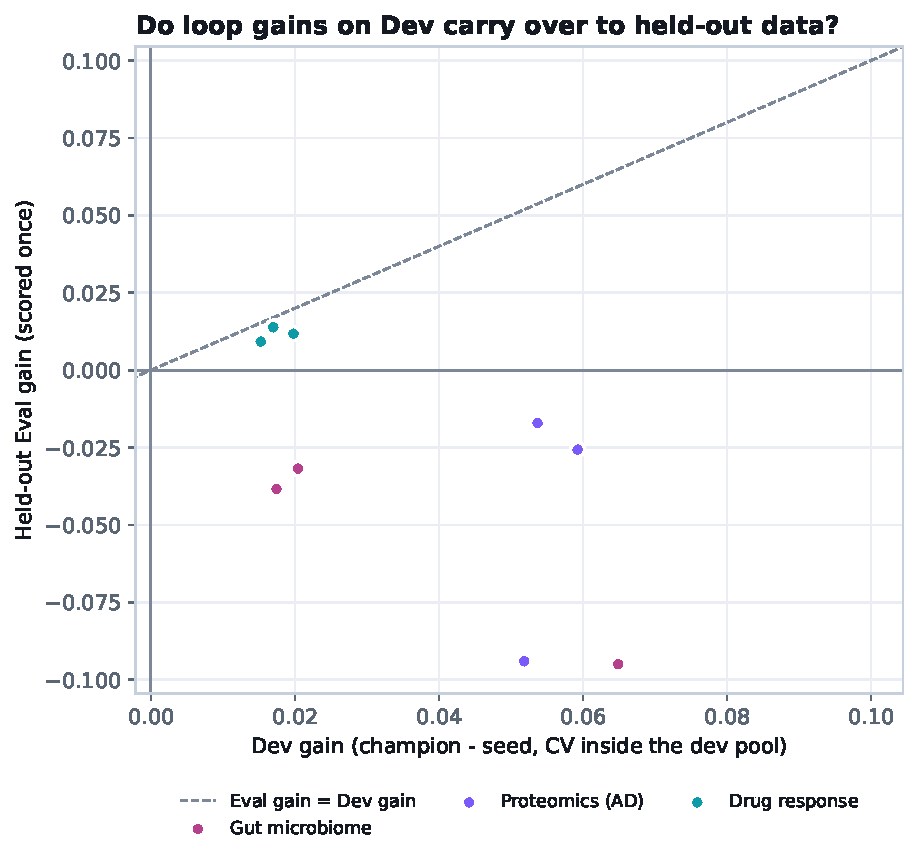
\includegraphics[width=0.6\linewidth]{fig1_dev_vs_eval_gain.pdf}
\caption{Dev gain vs.\ held-out Eval gain, one point per task and split. Dashed: Eval gain = Dev gain.}
\label{fig:dev-eval}
\end{figure}

\subsection{Feedback, not the LLM alone, produces the gains}\label{sec:baselines-results}
\Cref{tab:baselines} and \cref{fig:baselines} compare the loop with the three same-budget
baselines. A single LLM proposal was kept in only 15/36 splits (one failed to run) and changed Eval
by $+0.002$ on average. Twenty independent proposals without feedback did better ($+0.014$) but were
kept in only 25/36 splits: on neonatal seizure detection and ADHD (TDBRAIN), none of the 120
independent proposals across the three splits beat the seed on Dev, while the loop improved every
split of both tasks. The loop's own first two rounds on neonatal seizures also failed in every
split, and its first kept change came in round 3. On those tasks, the
improvement depended on the model seeing what had already failed. All 720 best-of-20 proposals ran
without crashing, so the low adoption rate reflects proposal quality, not a broken baseline.

Optuna, searching a space written with knowledge of the loop's findings, gained $+0.035$ on average
and matched the loop on several tasks, including both TDBRAIN tasks (MDD 0.946 vs.\ 0.954; ADHD
0.918 vs.\ 0.922) and ADHD-200 (0.650 vs.\ 0.665). It beat the loop on plasma AD (0.934 vs.\ 0.866)
and CSF AD (0.971 vs.\ 0.954).

\begin{table}[!tbp]
\centering
\caption{Held-out Eval score per arm with the same budget of 20 Dev evaluations (mean over 3
splits; bold = best non-seed arm). Every arm keeps a candidate only if it beats the seed on Dev.
Symbols as in \cref{tab:main}.}
\label{tab:baselines}
\footnotesize
% generated by paper/make_tables.py from results/robustness/baselines.csv -- do not edit
\begin{tabular}{lccccc}
\toprule
Task & Seed & One-shot & Best-of-20 & Optuna & Loop \\
\midrule
Abnormal EEG (TUAB) & 0.847 & 0.866 & 0.888 & 0.889 & \textbf{0.918} \\
MDD (TDBRAIN) & 0.850 & 0.864 & 0.884 & 0.946 & \textbf{0.954} \\
ADHD (TDBRAIN) & 0.785 & 0.785 & 0.785 & 0.918 & \textbf{0.922} \\
Schizophrenia (ASEEG) & 0.677 & 0.677 & 0.705 & 0.678 & \textbf{0.799} \\
Neonatal seizure (Helsinki) & 0.827 & 0.827 & 0.827 & 0.824 & \textbf{0.899} \\
Autism (ABIDE I)$^\dagger$ & 0.781 & 0.783 & \textbf{0.790} & 0.781 & 0.778 \\
ADHD (ADHD-200)$^{\dagger\S}$ & 0.572 & 0.570 & 0.627 & 0.650 & \textbf{0.665} \\
CRC (Baxter) & 0.795 & \textbf{0.789} & 0.787 & 0.759 & 0.740 \\
IBD (4 studies)$^\dagger$ & 0.721 & 0.737 & 0.755 & 0.713 & \textbf{0.755} \\
AD, plasma & 0.912 & 0.895 & 0.897 & \textbf{0.934} & 0.866 \\
AD, CSF$^\dagger$ & 0.913 & 0.913 & 0.891 & \textbf{0.971} & 0.954 \\
Drug response (PRISM)$^\ddagger$ & 0.149 & 0.149 & 0.149 & 0.148 & \textbf{0.160} \\
\bottomrule
\end{tabular}

\end{table}

\begin{figure}[!tbp]
\centering
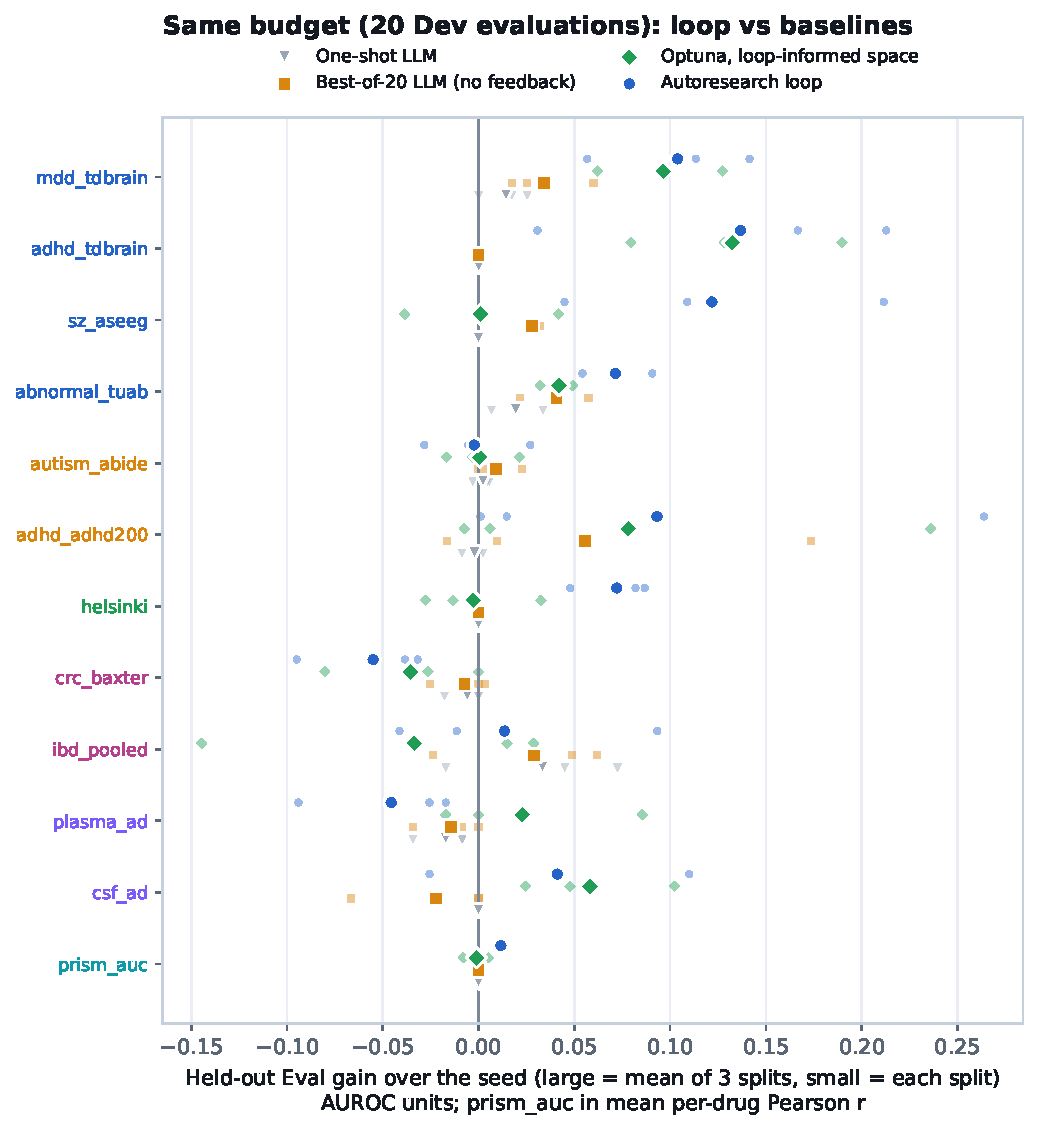
\includegraphics[width=0.75\linewidth]{fig7_baselines.pdf}
\caption{Held-out Eval gain over the seed for each arm with the same budget of 20 Dev
evaluations. Large markers: mean of 3 splits; small markers: individual splits.}
\label{fig:baselines}
\end{figure}

\subsection{Corrected statistics}\label{sec:stats-results}
\Cref{tab:stats} gives per-task gains with Holm-adjusted $p$-values, and \cref{tab:pooled} and
\cref{fig:meta} the pooled estimates. Against the seed, the loop's gain is Holm-significant on five
tasks (abnormal EEG $+0.071$, MDD $+0.104$, ADHD on TDBRAIN $+0.137$, neonatal seizure $+0.072$,
ADHD-200 $+0.093$) and its loss is significant on CRC ($-0.055$). The ADHD-200 result needs a
caveat: it is carried by split 1, whose seed scored below chance on Eval (0.453), and the split
gains are $+0.264$, $+0.001$ and $+0.015$; a $t$-test across the three splits gives $p=0.39$. Because
the per-task bootstrap treats fitted models as fixed, it does not capture this split-to-split
variation.

Pooled over 11 AUROC tasks, the loop gained $+0.052$ over the seed (95\% CI $+0.009$ to $+0.095$,
$p=0.023$), with high heterogeneity between tasks ($I^2=85\%$). Against Optuna the loop's pooled
advantage was $+0.017$ ($-0.017$ to $+0.051$, $p=0.29$), and against best-of-20 it was $+0.038$
($p=0.051$). Only two tasks show a Holm-significant advantage of the loop over Optuna: abnormal EEG
($+0.029$) and neonatal seizure detection ($+0.075$). The pooled gain over the seed also depends on
the TDBRAIN tasks, whose in-distribution signal does not transfer (\cref{sec:transfer}). Leaving
them out lowers it to $+0.037$ ($p=0.11$), and leaving out ADHD-200 as well lowers it to $+0.030$
($p=0.21$).

\begin{table}[!tbp]
\centering
\caption{Per-task Eval differences (mean over 3 splits) with Holm-adjusted two-sided bootstrap
$p$-values across the 12 tasks; bold = $p_\text{Holm}<0.05$. The bootstrap resamples subjects and
treats fitted models as fixed. Symbols as in \cref{tab:main}.}
\label{tab:stats}
\footnotesize
\setlength{\tabcolsep}{3pt}
\resizebox{\textwidth}{!}{% generated by paper/make_tables.py from results/stats_tasks.csv -- do not edit
\begin{tabular}{lrrrrrrrr}
\toprule
& \multicolumn{2}{c}{Loop $-$ seed} & \multicolumn{2}{c}{Optuna $-$ seed} & \multicolumn{2}{c}{Loop $-$ best-of-20} & \multicolumn{2}{c}{Loop $-$ Optuna} \\
\cmidrule(lr){2-3}\cmidrule(lr){4-5}\cmidrule(lr){6-7}\cmidrule(lr){8-9}
Task & gain & $p_\text{Holm}$ & gain & $p_\text{Holm}$ & gain & $p_\text{Holm}$ & gain & $p_\text{Holm}$ \\
\midrule
Abnormal EEG (TUAB) & \textbf{+0.071} & 0.012 & \textbf{+0.042} & 0.012 & \textbf{+0.031} & 0.012 & \textbf{+0.029} & 0.012 \\
MDD (TDBRAIN) & \textbf{+0.104} & 0.012 & \textbf{+0.096} & 0.012 & \textbf{+0.070} & 0.048 & +0.008 & 1.000 \\
ADHD (TDBRAIN) & \textbf{+0.137} & 0.012 & +0.132 & 0.090 & \textbf{+0.137} & 0.012 & +0.004 & 1.000 \\
Schizophrenia (ASEEG) & +0.122 & 0.165 & +0.001 & 1.000 & +0.094 & 0.182 & +0.121 & 0.504 \\
Neonatal seizure (Helsinki) & \textbf{+0.072} & 0.012 & $-$0.003 & 1.000 & \textbf{+0.072} & 0.012 & \textbf{+0.075} & 0.012 \\
Autism (ABIDE I)$^\dagger$ & $-$0.002 & 0.915 & +0.001 & 1.000 & $-$0.011 & 0.572 & $-$0.003 & 1.000 \\
ADHD (ADHD-200)$^\dagger$ & \textbf{+0.093} & 0.040 & +0.078 & 0.351 & +0.038 & 0.222 & +0.015 & 1.000 \\
CRC (Baxter) & \textbf{$-$0.055} & 0.040 & $-$0.036 & 0.568 & \textbf{$-$0.048} & 0.045 & $-$0.020 & 1.000 \\
IBD (4 studies)$^\dagger$ & +0.035 & 0.312 & $-$0.008 & 1.000 & +0.001 & 0.957 & +0.043 & 0.686 \\
AD, plasma & $-$0.046 & 0.312 & +0.023 & 1.000 & $-$0.031 & 0.344 & $-$0.068 & 0.220 \\
AD, CSF$^\dagger$ & +0.041 & 0.518 & +0.058 & 1.000 & +0.063 & 0.344 & $-$0.017 & 1.000 \\
Drug response (PRISM)$^\ddagger$ & +0.012 & 0.162 & $-$0.001 & 1.000 & +0.012 & 0.260 & +0.013 & 0.306 \\
\bottomrule
\end{tabular}
}
\end{table}

\begin{table}[!tbp]
\centering
\caption{Pooled Eval gain over the 11 AUROC tasks: equal-weight mean with a $t$-interval across
tasks (primary) and DerSimonian--Laird random effects (secondary). Sensitivity rows drop the two
TDBRAIN tasks (separate recruitment of cases and controls; no transfer to Mumtaz) and then also
ADHD-200 (gain carried by one split).}
\label{tab:pooled}
\footnotesize
\setlength{\tabcolsep}{4pt}
\resizebox{\textwidth}{!}{% generated by paper/make_tables.py from results/stats_pooled.json and stats_tasks.csv -- do not edit
\begin{tabular}{lcccccc}
\toprule
Comparison & $k$ & mean gain & 95\% CI & $p$ & random effects [95\% CI] & $I^2$ \\
\midrule
Loop vs.\ seed & 11 & +0.052 & [+0.009, +0.095] & 0.023 & +0.046 [+0.012, +0.080] & 85\% \\
Optuna vs.\ seed & 11 & +0.035 & [+0.000, +0.070] & 0.047 & +0.027 [+0.001, +0.052] & 70\% \\
Best-of-20 vs.\ seed & 11 & +0.014 & [$-$0.003, +0.031] & 0.090 & +0.012 [$-$0.003, +0.026] & 74\% \\
One-shot vs.\ seed & 11 & +0.002 & [$-$0.005, +0.010] & 0.457 & +0.003 [$-$0.002, +0.008] & 26\% \\
Loop vs.\ Optuna & 11 & +0.017 & [$-$0.017, +0.051] & 0.290 & +0.015 [$-$0.004, +0.034] & 67\% \\
Loop vs.\ best-of-20 & 11 & +0.038 & [$-$0.000, +0.076] & 0.051 & +0.028 [+0.003, +0.053] & 83\% \\
Loop vs.\ one-shot & 11 & +0.050 & [+0.009, +0.090] & 0.022 & +0.041 [+0.011, +0.072] & 85\% \\
\midrule
\multicolumn{7}{l}{\emph{Sensitivity: leaving out tasks with suspect in-distribution gains}} \\
Loop vs.\ seed, without TDBRAIN & 9 & +0.037 & [$-$0.010, +0.084] & 0.107 & & \\
Loop vs.\ seed, without TDBRAIN, ADHD-200 & 8 & +0.030 & [$-$0.021, +0.081] & 0.210 & & \\
Loop vs.\ Optuna, without TDBRAIN & 9 & +0.019 & [$-$0.024, +0.062] & 0.328 & & \\
Loop vs.\ Optuna, without TDBRAIN, ADHD-200 & 8 & +0.020 & [$-$0.030, +0.070] & 0.376 & & \\
\bottomrule
\end{tabular}
}
\end{table}

\begin{figure}[!tbp]
\centering
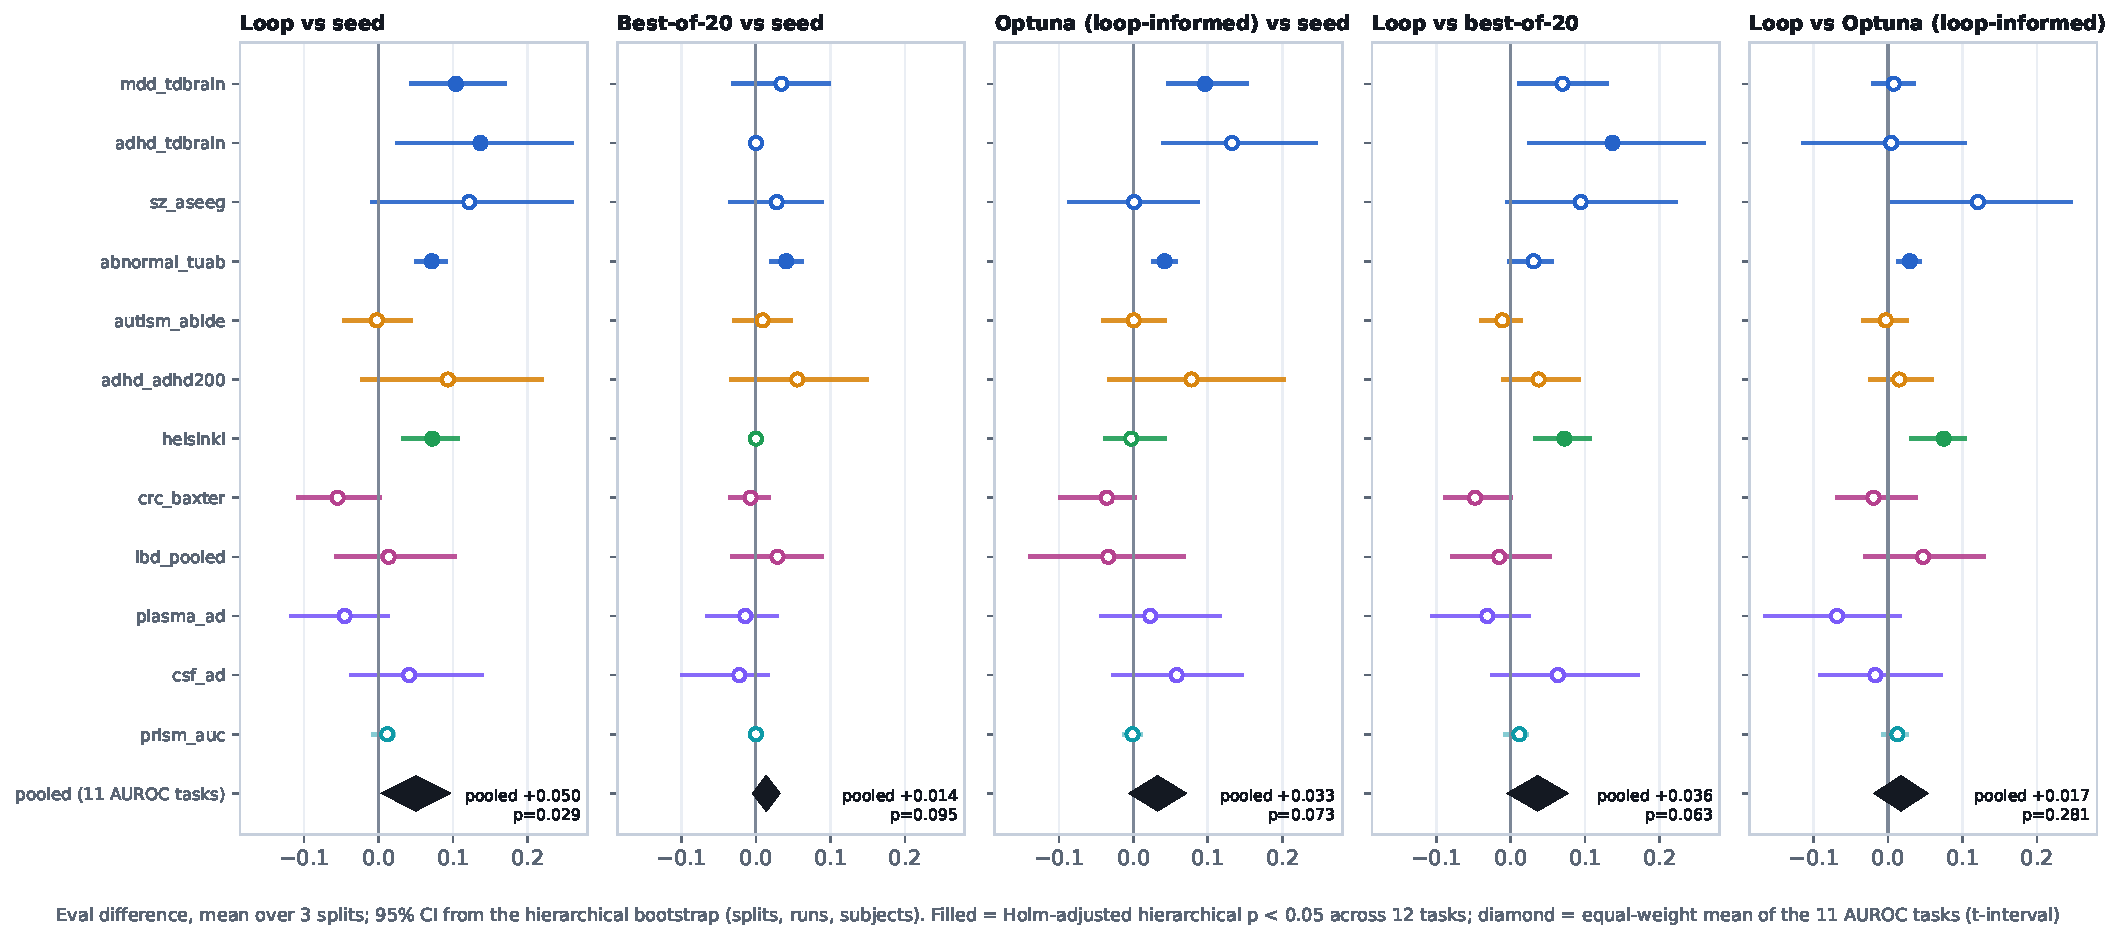
\includegraphics[width=\linewidth]{fig8_meta_forest.pdf}
\caption{Per-task Eval differences with 95\% CIs (task-level subject bootstrap) for five
comparisons. Filled: Holm-adjusted $p<0.05$ across 12 tasks (as reported by \texttt{core/stats.py};
the significant tasks are the same as in \cref{tab:stats}). Diamond: equal-weight mean of the 11
AUROC tasks with $t$-interval.}
\label{fig:meta}
\end{figure}

\subsection{Run-to-run variance}\label{sec:variance}
Repeating the loop on the same split changed the Eval gain by less than drawing a different split
did (\cref{fig:variance}). Across three independent loops on split 1, the standard deviation of the
Eval gain was 0.011--0.044 (median 0.016), compared with 0.002--0.084 (median 0.042) across splits;
run-to-run variation was smaller for six of the seven tasks (drug response is the exception,
0.016 vs.\ 0.002). The sign of the gain was stable on three tasks (IBD, MDD and schizophrenia,
positive in all three repeats), never positive on plasma AD, and flipped between repeats on CRC,
CSF AD and drug response. Repeats were not run for abnormal EEG, neonatal seizure, ADHD on
TDBRAIN, ABIDE or ADHD-200 because of their compute cost; this includes the two tasks with the
clearest gains.

\begin{figure}[!tbp]
\centering
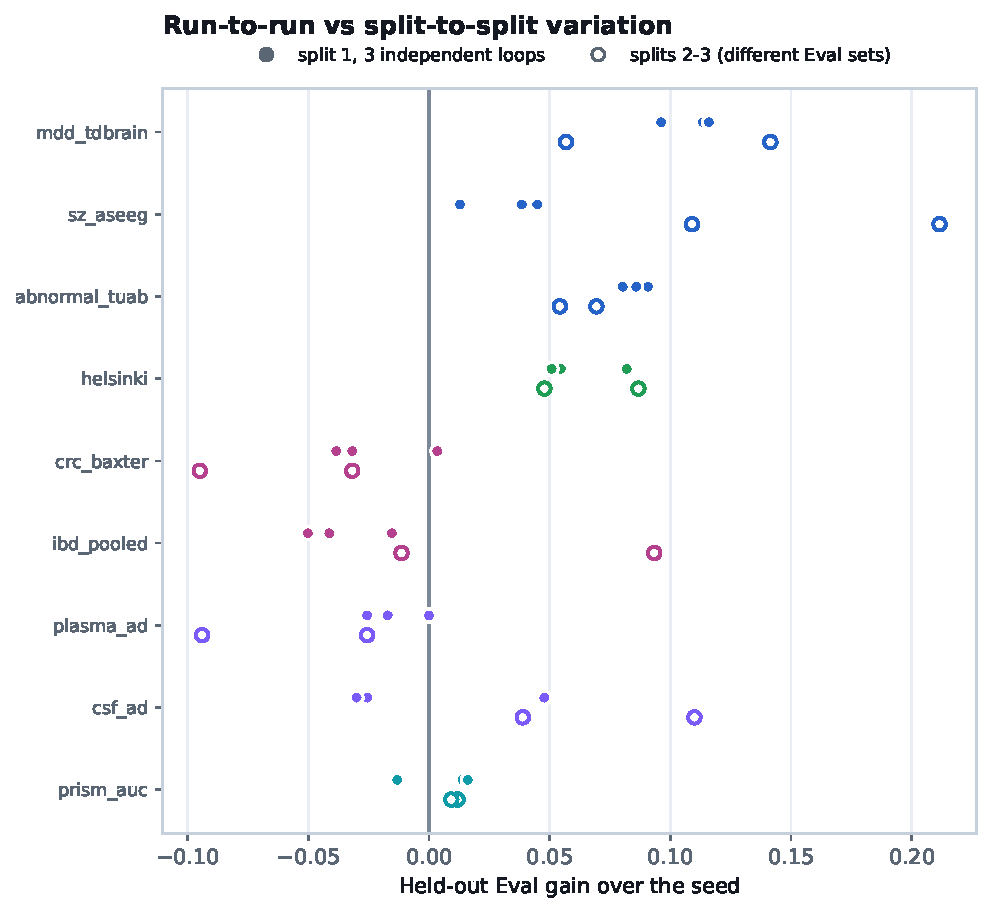
\includegraphics[width=0.65\linewidth]{fig9_variance.pdf}
\caption{Eval gain of three independent loops on split 1 (filled) and of the loops on splits 2--3
(hollow), for the seven tasks with repeats.}
\label{fig:variance}
\end{figure}

\subsection{The loop finds shortcuts when they exist}\label{sec:shortcuts}
Under protocol v1, every ADHD-200 and ABIDE champion and every pooled-IBD champion referenced
non-biological inputs in code: site, age and sex on ADHD-200; site, age, sex and head motion on
ABIDE; and study identity on pooled IBD (\cref{fig:shortcuts}). These shortcuts carry substantial
signal on their own. With no biological input, site plus age and sex reach a pooled Eval AUROC of
0.775 on ADHD-200, close to the v1 champion's 0.813; study identity alone reaches 0.691 on pooled
IBD and site alone 0.727 on CSF AD. Rescored within site, the v1 ADHD-200 champion drops from 0.813
to 0.731, close to the v2 champion on the same split (0.717).

Within-site scoring removes the site shortcut (site-only models score 0.500 within site) but not
the demographic one: on ADHD-200, age and sex alone still give a within-site AUROC of 0.647,
because ADHD and control groups differ in sex and age inside sites. The v2 ADHD-200 champion
(0.665) is only slightly above this floor. Connectivity is known to encode sex and age, so v2's
removal of these \emph{inputs} does not guarantee that the model does not use the corresponding
\emph{signal}.

\begin{figure}[!tbp]
\centering
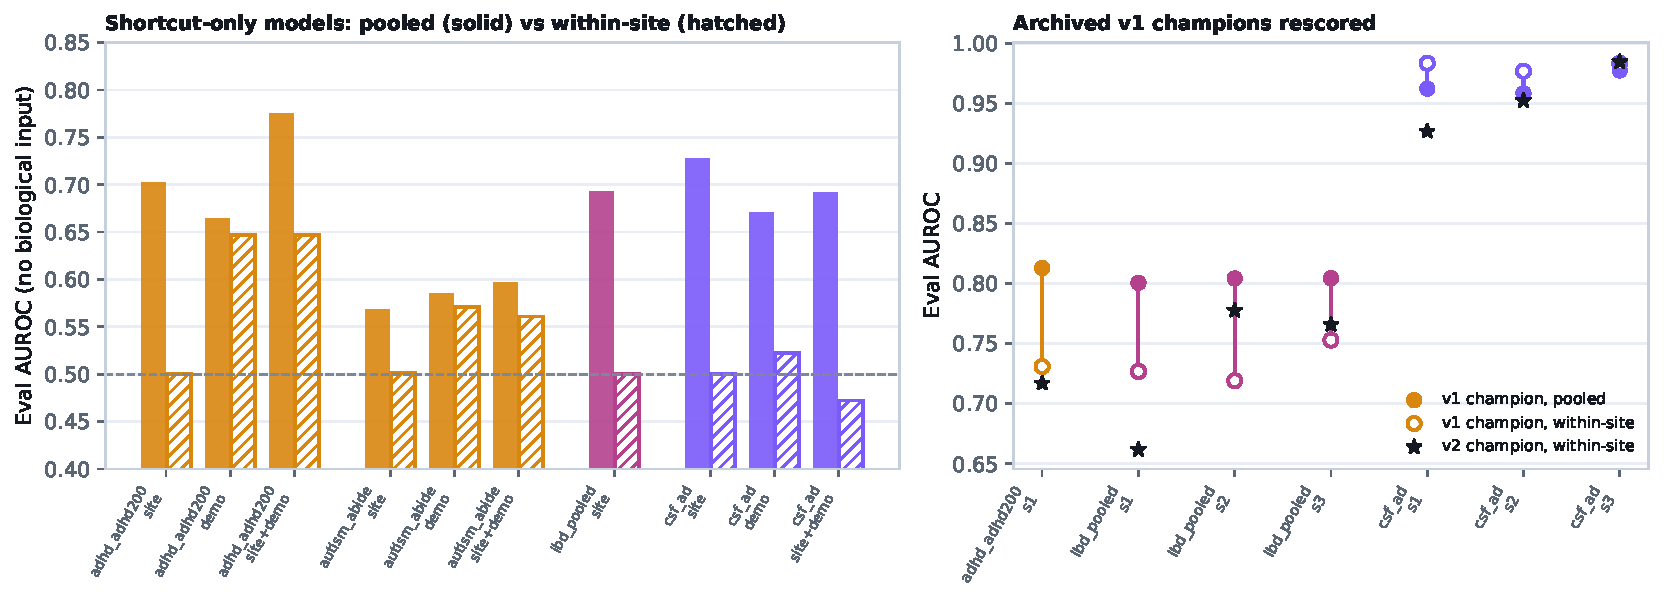
\includegraphics[width=\linewidth]{fig10_shortcuts.pdf}
\caption{Left: Eval AUROC of shortcut-only models (no biological input), pooled (solid) and
within site (hatched). Right: archived v1 champions rescored with the pooled and the within-site
metric, with the v2 champion on the same split.}
\label{fig:shortcuts}
\end{figure}

\subsection{In-distribution gains did not transfer to other cohorts}\label{sec:transfer}
\Cref{tab:external} and \cref{fig:transfer} apply the seed and champion of each split, unchanged,
to independent datasets. Only abnormal EEG transferred: on the official TUAB evaluation split the
champion improved on the seed in all three splits ($+0.052$ to $+0.067$, all CIs excluding zero;
AUROC 0.867 $\to$ 0.928). That split comes from the same hospital and protocol, so it is a
near-in-distribution check rather than an external cohort.

On depression, the TDBRAIN seed was \emph{inverted} on the Mumtaz cohort (AUROC 0.25--0.29), and
the champions reached 0.28--0.62 (mean 0.494). The large numerical gain moves an inverted model to
chance. It is evidence that the TDBRAIN case/control signal is specific to that dataset,
plausibly reflecting separate recruitment and recording of patients and controls, not that a
transferable depression marker was found. On schizophrenia, the champion was worse than the
seed on the MSU adolescent cohort in all three splits ($-0.016$, $-0.162$, $-0.296$; mean AUROC
0.696 $\to$ 0.538) and mixed on the small RepOD cohort (all CIs include zero). On CRC, the
champion lost on Eval and on all four external cohorts on average ($-0.008$ to $-0.053$).

\begin{figure}[!tbp]
\centering
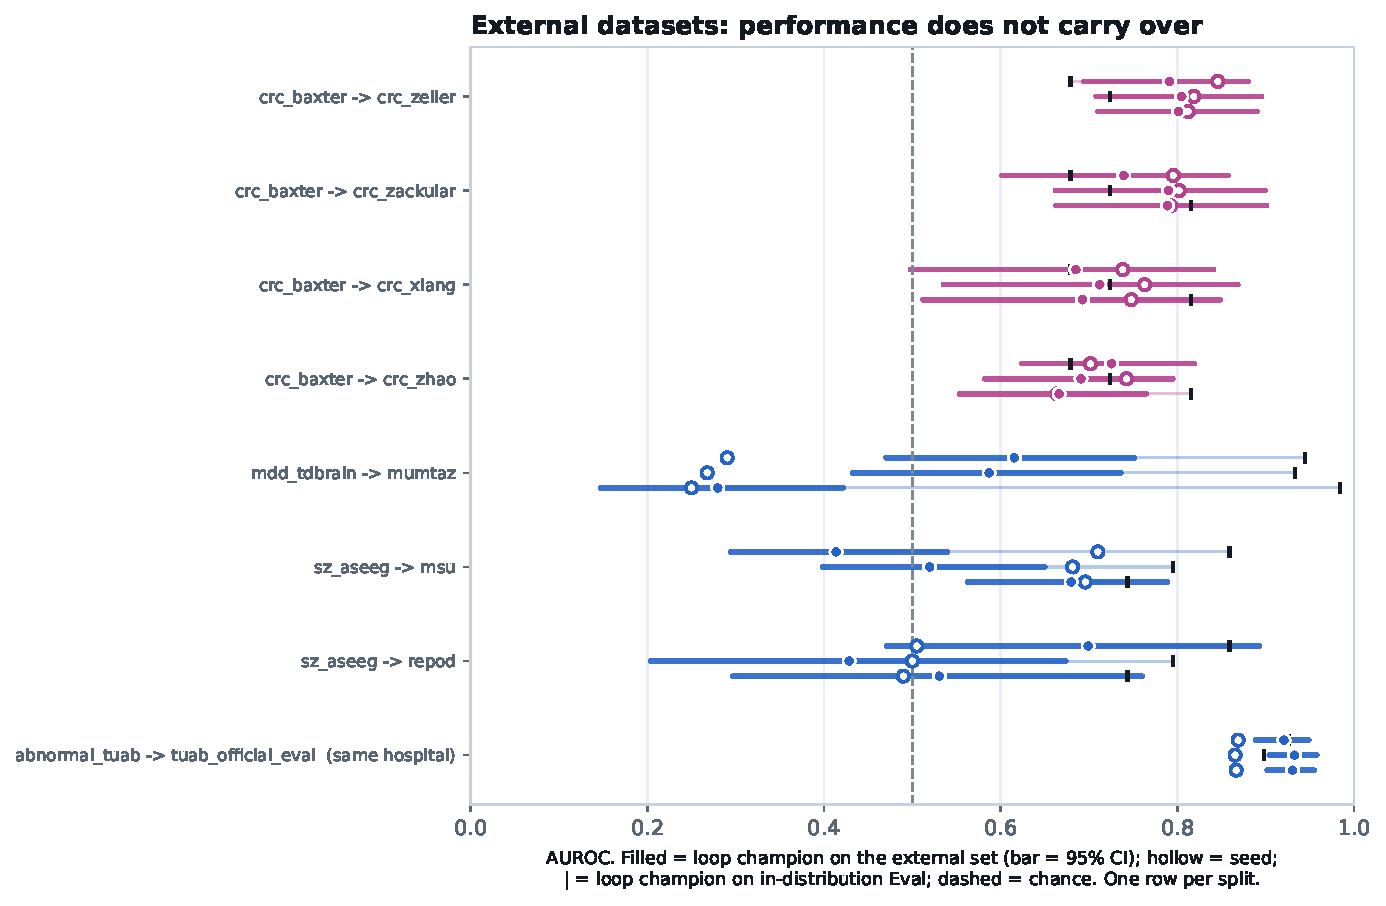
\includegraphics[width=0.85\linewidth]{fig11_transfer.pdf}
\caption{In-distribution Eval gain vs.\ gain on an external dataset for the same model, one point
per split and external set. Dashed: equal gain.}
\label{fig:transfer}
\end{figure}

\begin{table}[!tbp]
\centering
\caption{External datasets: seed and champion applied unchanged; 95\% CI from the paired bootstrap.}
\label{tab:external}
\footnotesize
% generated by paper/make_tables.py from projects/*/runs/*/s*/final_scores.json -- do not edit
\begin{tabular}{llccccc}
\toprule
Task & External set & split & seed & champion & gain & 95\% CI \\
\midrule
Abnormal EEG (TUAB) & TUAB official eval & 1 & 0.867 & 0.930 & +0.064 & [+0.034, +0.096] \\
 &  & 2 & 0.865 & 0.933 & +0.067 & [+0.035, +0.104] \\
 &  & 3 & 0.869 & 0.921 & +0.052 & [+0.020, +0.084] \\
\addlinespace
MDD (TDBRAIN) & Mumtaz 2016 & 1 & 0.250 & 0.280 & +0.030 & [$-$0.123, +0.190] \\
 &  & 2 & 0.268 & 0.587 & +0.319 & [+0.120, +0.518] \\
 &  & 3 & 0.290 & 0.615 & +0.325 & [+0.154, +0.502] \\
\addlinespace
Schizophrenia (ASEEG) & MSU & 1 & 0.696 & 0.680 & $-$0.016 & [$-$0.108, +0.077] \\
 &  & 2 & 0.681 & 0.520 & $-$0.162 & [$-$0.276, $-$0.043] \\
 &  & 3 & 0.710 & 0.414 & $-$0.296 & [$-$0.438, $-$0.147] \\
 & RepOD & 1 & 0.490 & 0.531 & +0.041 & [$-$0.182, +0.262] \\
 &  & 2 & 0.500 & 0.429 & $-$0.071 & [$-$0.231, +0.109] \\
 &  & 3 & 0.505 & 0.699 & +0.194 & [$-$0.052, +0.448] \\
\addlinespace
CRC (Baxter) & Zeller & 1 & 0.813 & 0.801 & $-$0.011 & [$-$0.058, +0.035] \\
 &  & 2 & 0.818 & 0.805 & $-$0.013 & [$-$0.054, +0.024] \\
 &  & 3 & 0.846 & 0.791 & $-$0.055 & [$-$0.114, $-$0.002] \\
 & Zackular & 1 & 0.792 & 0.789 & $-$0.003 & [$-$0.053, +0.053] \\
 &  & 2 & 0.802 & 0.790 & $-$0.012 & [$-$0.055, +0.034] \\
 &  & 3 & 0.796 & 0.739 & $-$0.056 & [$-$0.144, +0.024] \\
 & Xiang & 1 & 0.748 & 0.693 & $-$0.055 & [$-$0.126, $-$0.007] \\
 &  & 2 & 0.763 & 0.712 & $-$0.051 & [$-$0.163, +0.054] \\
 &  & 3 & 0.738 & 0.685 & $-$0.053 & [$-$0.133, +0.012] \\
 & Zhao & 1 & 0.664 & 0.666 & +0.002 & [$-$0.029, +0.031] \\
 &  & 2 & 0.742 & 0.691 & $-$0.051 & [$-$0.112, +0.006] \\
 &  & 3 & 0.702 & 0.726 & +0.024 & [$-$0.043, +0.091] \\
\bottomrule
\end{tabular}

\end{table}

\subsection{Reported Eval scores do not depend on Eval-batch statistics}\label{sec:audit}
All 36 seeds were exactly inductive. Of the 36 champions, 9 had a batch-dependent
\texttt{featurize} and 11 returned batch-relative outputs (ranks). Scoring each Eval chunk inside a
reference batch built from the dev pool changed champion Eval scores by $+0.001$ on average (worst
case: CSF AD split 1, $-0.024$), so the reported scores are not inflated by statistics of the
held-out set (\cref{fig:audit}). Scoring chunks in isolation, without a reference batch, cost
rank-output champions up to 0.29 AUROC (CSF AD split 1: 0.927 $\to$ 0.637). Such pipelines would
need a reference cohort to score a single patient.

\begin{figure}[!tbp]
\centering
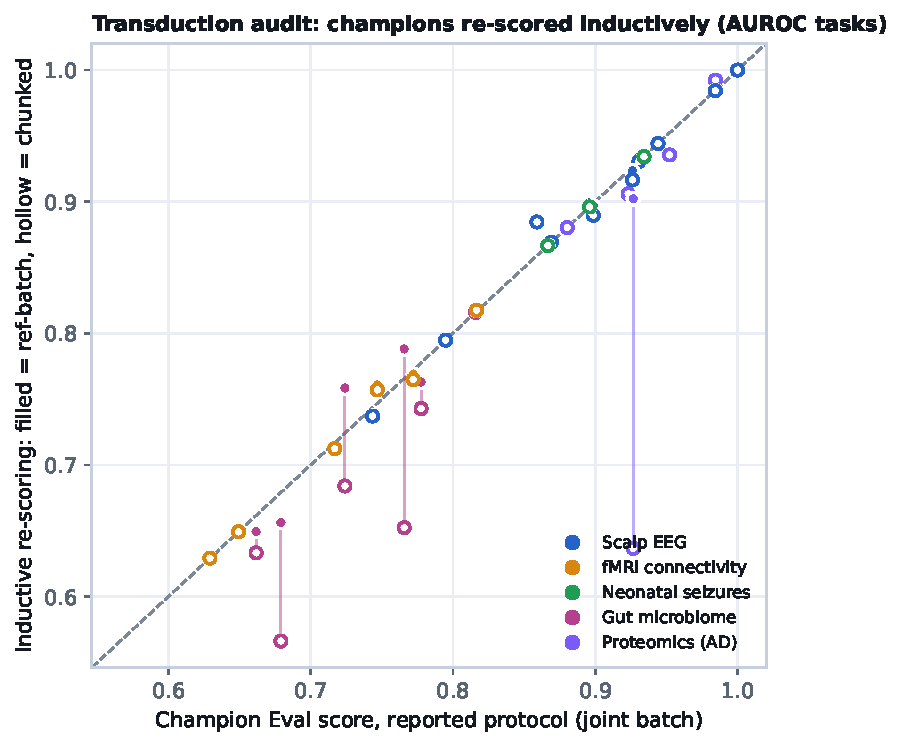
\includegraphics[width=0.5\linewidth]{fig12_audit.pdf}
\caption{Transduction audit of the champions (AUROC tasks). $x$: Eval score as reported (joint
batch). Filled: reference-batch score; hollow: chunks scored in isolation. Points on the diagonal
do not depend on the Eval batch.}
\label{fig:audit}
\end{figure}

\subsection{What the loop built}\label{sec:families}
\Cref{fig:families} summarizes the feature and model families in the final champions as
\emph{declared by the LLM} in each kept round; it is a self-report, not an analysis of the code.
Champions typically extended the seed's representation with domain features rather than replacing
the model. Examples include finer clinical frequency sub-bands, aperiodic slope, connectivity,
complexity measures and covariance (Riemannian) features for EEG; per-neonate and per-channel
background normalization and multi-scale temporal context for neonatal seizures; log-ratio
transforms and batch correction for microbiome data; and known AD proteins and pathway
aggregates for proteomics. Ensembles of a linear model with gradient boosting or kernel methods
were common.

\begin{figure}[!tbp]
\centering
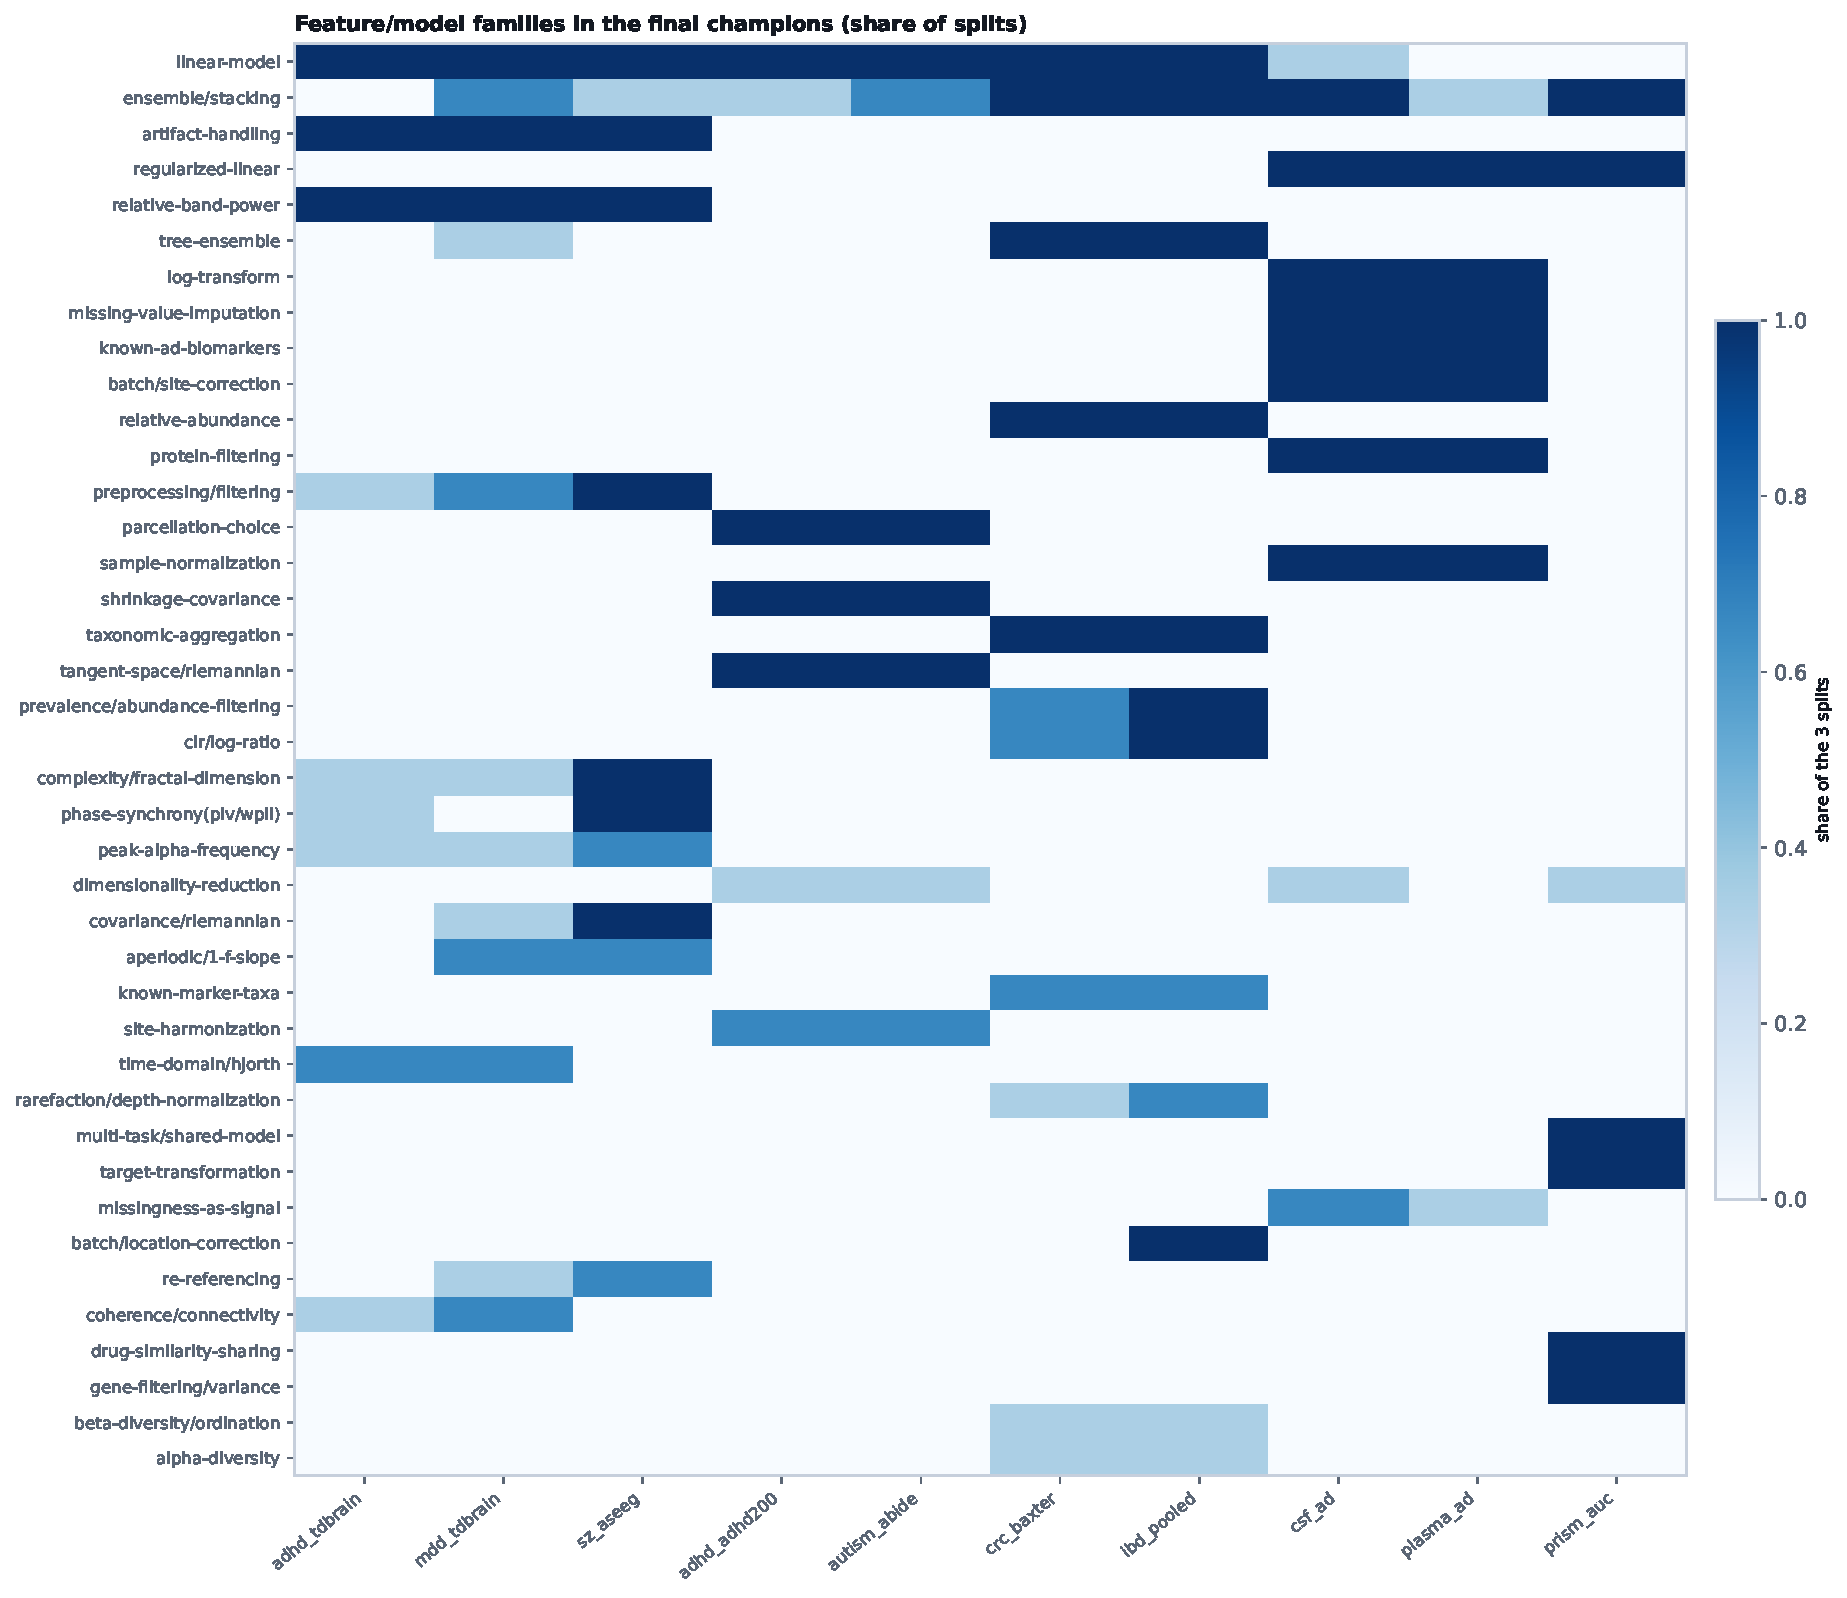
\includegraphics[width=\linewidth,height=0.75\textheight,keepaspectratio]{fig4_families.pdf}
\caption{Feature/model families in the final champions (share of the 3 splits), as declared by the LLM.}
\label{fig:families}
\end{figure}

% ===========================================================================================
\section{Discussion}\label{sec:discussion}
% ===========================================================================================
\paragraph{When the loop helped.} The clearest gains came on the two signal-processing tasks with
large or well-annotated data and clinically meaningful labels: abnormal EEG, where the gain held
on the official evaluation split, and neonatal seizure detection. These were also the only tasks
where the loop beat a tuned, loop-informed Optuna search. On both, independent LLM proposals almost
never beat the seed, and the loop's first two rounds failed too; improvement came from proposals
that built on what had already been tried. Feedback, not the LLM's prior knowledge alone, is the
active ingredient.

\paragraph{When it did not.} On most other tasks the loop was not reliably better than ordinary
search, and on three it was worse than the seed on held-out data despite consistent Dev gains. The
loop's largest in-distribution gains, on TDBRAIN depression and ADHD, were matched by Optuna and
did not transfer to an external cohort, which points to dataset-specific signal that any optimizer
would find. The schizophrenia gain reversed on an external cohort. When site and demographics were
available, the loop used them, as an optimizer should.

\paragraph{Implications.} For anyone running such a loop, the Dev curve says little: Dev improved
in every run, and the correlation between Dev and Eval gains was $0.38$. A held-out set scored once,
a same-budget non-LLM baseline, shortcut-only models on the same data, and an external cohort each
changed our reading of at least one task. The loop is best seen as a strong, cheap search
procedure whose outputs need the same validation as any other model. That procedure is also
especially good at finding whatever the evaluation rewards.

\paragraph{Clinical comparison.} Our numbers are not directly comparable to published results:
within-site AUROC is stricter than the pooled metrics usually reported for ABIDE and ADHD-200, and
the Helsinki literature uses different annotation rules and leave-one-out evaluation. Where a rough
comparison is possible, the champions were at or below the literature: on Helsinki, 0.899 vs.\
about 0.955 concatenated AUROC for an SVM baseline \citep{tapani2022} and 0.98 for a CNN trained on
a different cohort \citep{hogan2025}; on CRC, the seed (0.795) already matched the MicrobiomeHD
random-forest baseline \citep{duvallet2017} and the loop made it worse.

\subsection{Limitations}\label{sec:limitations}
\begin{itemize}
  \item \textbf{Small Eval sets.} Several tasks have 20--43 held-out subjects per split (plasma AD 22,
        schizophrenia 25, neonatal seizure 20 neonates, CSF AD 34, ADHD on TDBRAIN 43), so per-task
        CIs are wide and one split reached AUROC 1.000 (ADHD on TDBRAIN, split 2).
  \item \textbf{Three overlapping splits.} The Eval sets share subjects; the per-task bootstrap does
        not capture split-to-split or run-to-run variation, and repeats were run for only 7 of 12
        tasks, not including abnormal EEG or neonatal seizure.
  \item \textbf{One model and one setting.} All loops used one LLM at one reasoning effort and one
        budget (20 rounds, 1{,}500\,s per candidate on CPUs), which favours light models.
  \item \textbf{Baseline design.} The Optuna search spaces were written after the main study and
        include ideas from the loop. This makes the comparison conservative for the loop, but it
        does not test what a domain expert would write without that information.
  \item \textbf{Dataset confounds.} TDBRAIN patients and controls were recruited and recorded
        separately; age is controlled by matching but state or protocol differences cannot be
        excluded. ADHD-200 groups differ in sex and age within sites. The ASEEG channel order is
        undocumented and was inferred from data (correlation-structure match to labelled RepOD
        recordings, $r=0.855$). The CSF label is clinical diagnosis; the plasma set is from a single
        centre.
  \item \textbf{Researcher degrees of freedom.} Protocol v2 was designed after seeing v1. We report
        v1 as a finding (\cref{sec:shortcuts}), but the choice of v2 rules was informed by it.
  \item \textbf{Self-reported families.} \Cref{fig:families} reflects what the LLM said it did.
\end{itemize}

\section{Conclusion}\label{sec:conclusion}
An LLM autoresearch loop with feedback improved held-out performance over a simple seed on most of
12 biomedical tasks. Its advantage over 20 independent LLM proposals came from feedback, and its
advantage over a tuned non-LLM search was significant on only two signal-processing tasks. The same
loop found and used site and demographic shortcuts when they were available, and its gains on
psychiatric EEG did not transfer to external cohorts. Development-score gains from such a loop
should be read as a hypothesis to be tested on held-out, shortcut-free and external data, not as
evidence of a better biomarker.

\section*{Data and code availability}
Code, all loop records (every round's rationale, declared families, score and failure reason), the
champions, Eval predictions and the robustness analyses are available at
\url{https://github.com/radnyees/justautoeverything}. Raw data are not redistributed (TDBRAIN data use
agreement, TUH/NEDC terms, CC BY-NC licences); \texttt{projects/*/data/} contains scripts that
download and preprocess every dataset from its original source (\texttt{docs/references.md}).
Compute: Modal CPU containers, \$117.65 in total (\$60.0 main study, \$57.7 robustness analyses);
LLM calls used a Claude subscription and are not included in that figure.

\FloatBarrier
\bibliographystyle{plainnat}
\bibliography{references}

\clearpage
% ===========================================================================================
\appendix
\section{Per-run results}\label{app:per-run}
% ===========================================================================================

\begin{table}[htbp]
\centering
\caption{Every run. ``failed'' = timeouts + crashes. Eval gain CI and one-sided $p$ from the
subject-clustered paired bootstrap (2,000 resamples).}
\label{tab:per-run}
\footnotesize
\setlength{\tabcolsep}{4pt}
\resizebox{\textwidth}{!}{% generated by paper/make_tables.py from results/summary_runs.csv -- do not edit
\begin{tabular}{lcccccccc}
\toprule
Task & split & rounds & kept & failed & Dev gain & Eval gain & 95\% CI & $p$ (one-sided) \\
\midrule
Abnormal EEG (TUAB) & 1 & 20 & 11 & 0 & +0.068 & +0.091 & [+0.067, +0.116] & $<$0.001 \\
 & 2 & 20 & 9 & 1 & +0.068 & +0.069 & [+0.045, +0.096] & $<$0.001 \\
 & 3 & 20 & 10 & 3 & +0.071 & +0.054 & [+0.033, +0.076] & $<$0.001 \\
\addlinespace
MDD (TDBRAIN) & 1 & 20 & 7 & 0 & +0.089 & +0.113 & [+0.033, +0.203] & $<$0.001 \\
 & 2 & 20 & 11 & 0 & +0.093 & +0.141 & [+0.038, +0.258] & 0.001 \\
 & 3 & 20 & 6 & 0 & +0.118 & +0.057 & [$-$0.005, +0.132] & 0.042 \\
\addlinespace
ADHD (TDBRAIN) & 1 & 20 & 6 & 0 & +0.132 & +0.031 & [$-$0.031, +0.118] & 0.186 \\
 & 2 & 20 & 10 & 0 & +0.185 & +0.167 & [+0.060, +0.303] & $<$0.001 \\
 & 3 & 20 & 11 & 0 & +0.136 & +0.213 & [+0.045, +0.392] & 0.004 \\
\addlinespace
Schizophrenia (ASEEG) & 1 & 20 & 6 & 0 & +0.113 & +0.045 & [$-$0.104, +0.201] & 0.307 \\
 & 2 & 20 & 10 & 0 & +0.048 & +0.212 & [+0.035, +0.420] & 0.012 \\
 & 3 & 20 & 8 & 0 & +0.071 & +0.109 & [$-$0.019, +0.292] & 0.065 \\
\addlinespace
Neonatal seizure (Helsinki) & 1 & 20 & 11 & 0 & +0.126 & +0.082 & [+0.034, +0.121] & 0.002 \\
 & 2 & 20 & 10 & 0 & +0.093 & +0.048 & [+0.015, +0.106] & 0.003 \\
 & 3 & 20 & 7 & 1 & +0.122 & +0.087 & [+0.045, +0.171] & $<$0.001 \\
\addlinespace
Autism (ABIDE I)$^\dagger$ & 1 & 19 & 7 & 1 & +0.054 & $-$0.028 & [$-$0.091, +0.033] & 0.816 \\
 & 2 & 11 & 1 & 0 & +0.031 & +0.027 & [$-$0.038, +0.094] & 0.210 \\
 & 3 & 20 & 10 & 0 & +0.057 & $-$0.005 & [$-$0.067, +0.055] & 0.564 \\
\addlinespace
ADHD (ADHD-200)$^{\dagger\S}$ & 1 & 20 & 5 & 0 & +0.061 & +0.264 & [+0.129, +0.344] & $<$0.001 \\
 & 2 & 20 & 5 & 0 & +0.111 & +0.001 & [$-$0.075, +0.081] & 0.491 \\
 & 3 & 20 & 7 & 0 & +0.054 & +0.015 & [$-$0.062, +0.113] & 0.306 \\
\addlinespace
CRC (Baxter) & 1 & 20 & 5 & 0 & +0.017 & $-$0.038 & [$-$0.096, +0.019] & 0.922 \\
 & 2 & 20 & 6 & 0 & +0.020 & $-$0.032 & [$-$0.091, +0.021] & 0.873 \\
 & 3 & 20 & 10 & 0 & +0.065 & $-$0.095 & [$-$0.185, $-$0.012] & 0.991 \\
\addlinespace
IBD (4 studies)$^\dagger$ & 1 & 20 & 7 & 1 & +0.042 & +0.065 & [$-$0.006, +0.134] & 0.035 \\
 & 2 & 20 & 6 & 1 & +0.035 & +0.031 & [$-$0.038, +0.104] & 0.185 \\
 & 3 & 20 & 9 & 1 & +0.054 & +0.008 & [$-$0.054, +0.070] & 0.406 \\
\addlinespace
AD, plasma & 1 & 20 & 6 & 0 & +0.054 & $-$0.017 & [$-$0.106, +0.038] & 0.790 \\
 & 2 & 20 & 8 & 0 & +0.052 & $-$0.094 & [$-$0.217, +0.000] & 0.999 \\
 & 3 & 20 & 6 & 0 & +0.059 & $-$0.026 & [$-$0.125, +0.067] & 0.772 \\
\addlinespace
AD, CSF$^\dagger$ & 1 & 20 & 10 & 0 & +0.108 & $-$0.026 & [$-$0.155, +0.096] & 0.692 \\
 & 2 & 20 & 6 & 1 & +0.085 & +0.039 & [$-$0.068, +0.168] & 0.257 \\
 & 3 & 20 & 8 & 0 & +0.057 & +0.110 & [+0.014, +0.250] & 0.015 \\
\addlinespace
Drug response (PRISM)$^\ddagger$ & 1 & 20 & 9 & 0 & +0.017 & +0.014 & [$-$0.004, +0.032] & 0.055 \\
 & 2 & 20 & 9 & 0 & +0.020 & +0.012 & [$-$0.003, +0.027] & 0.059 \\
 & 3 & 20 & 10 & 0 & +0.015 & +0.009 & [$-$0.008, +0.026] & 0.174 \\
\bottomrule
\end{tabular}
}
\end{table}

\begin{figure}[htbp]
\centering
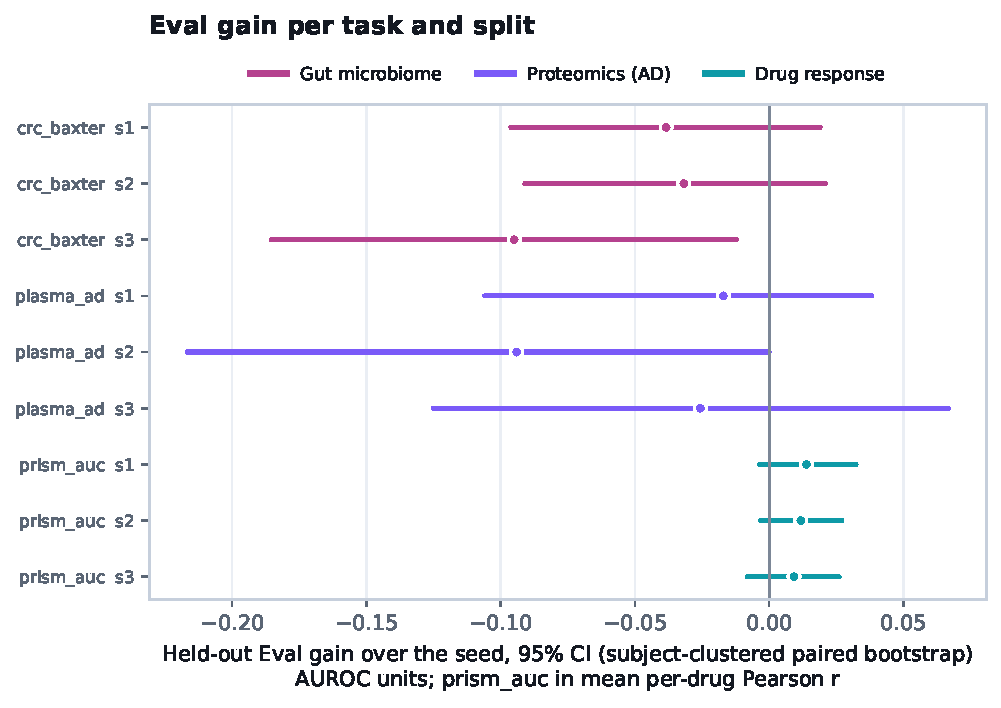
\includegraphics[width=\linewidth,height=0.8\textheight,keepaspectratio]{fig2_eval_gain_forest.pdf}
\caption{Held-out Eval gain over the seed with 95\% CI (subject-clustered paired bootstrap), per task and split.}
\label{fig:forest}
\end{figure}

\begin{figure}[htbp]
\centering
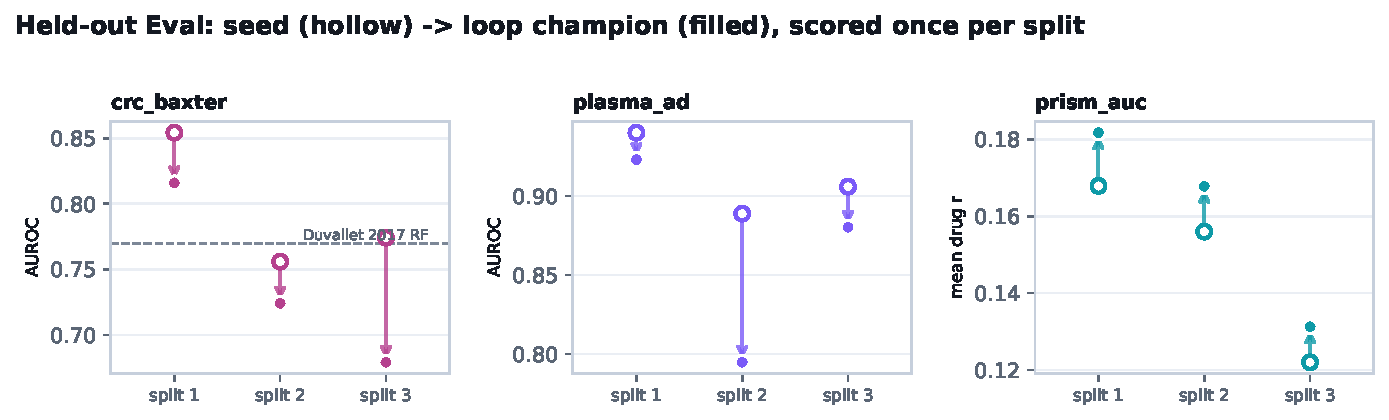
\includegraphics[width=\linewidth]{fig6_before_after.pdf}
\caption{Held-out Eval score of the seed (hollow) and the loop champion (filled), scored once per
split. Dashed lines: published results on the same dataset (different protocols; see
\cref{sec:discussion}).}
\label{fig:before-after}
\end{figure}

\begin{figure}[htbp]
\centering
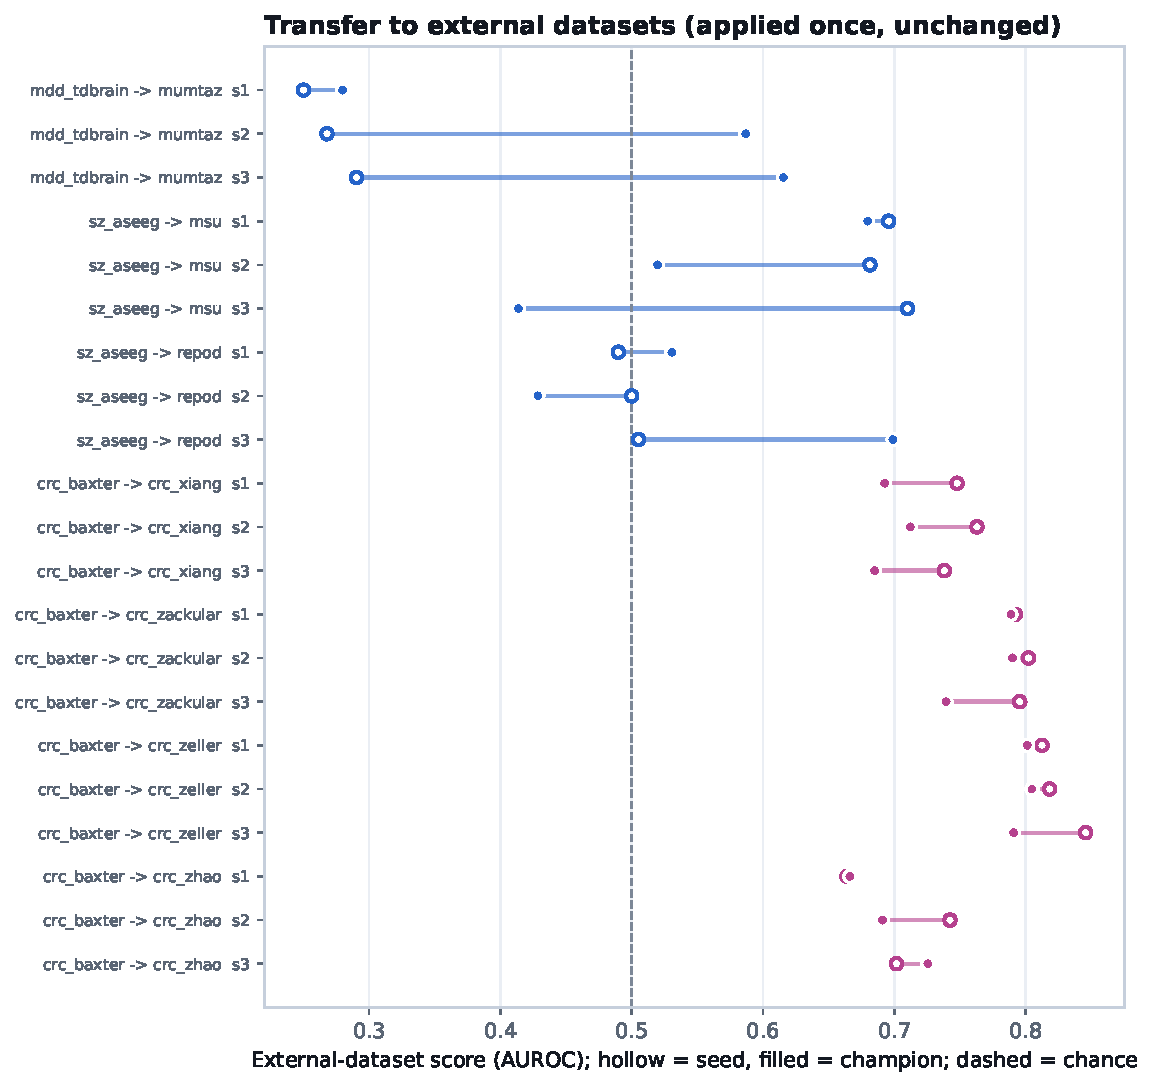
\includegraphics[width=0.85\linewidth]{fig5_external_transfer.pdf}
\caption{Transfer to external datasets. Hollow: seed; filled: champion; dashed: chance.}
\label{fig:external}
\end{figure}

\section{Loop trajectories}\label{app:trajectories}

\begin{figure}[htbp]
\centering
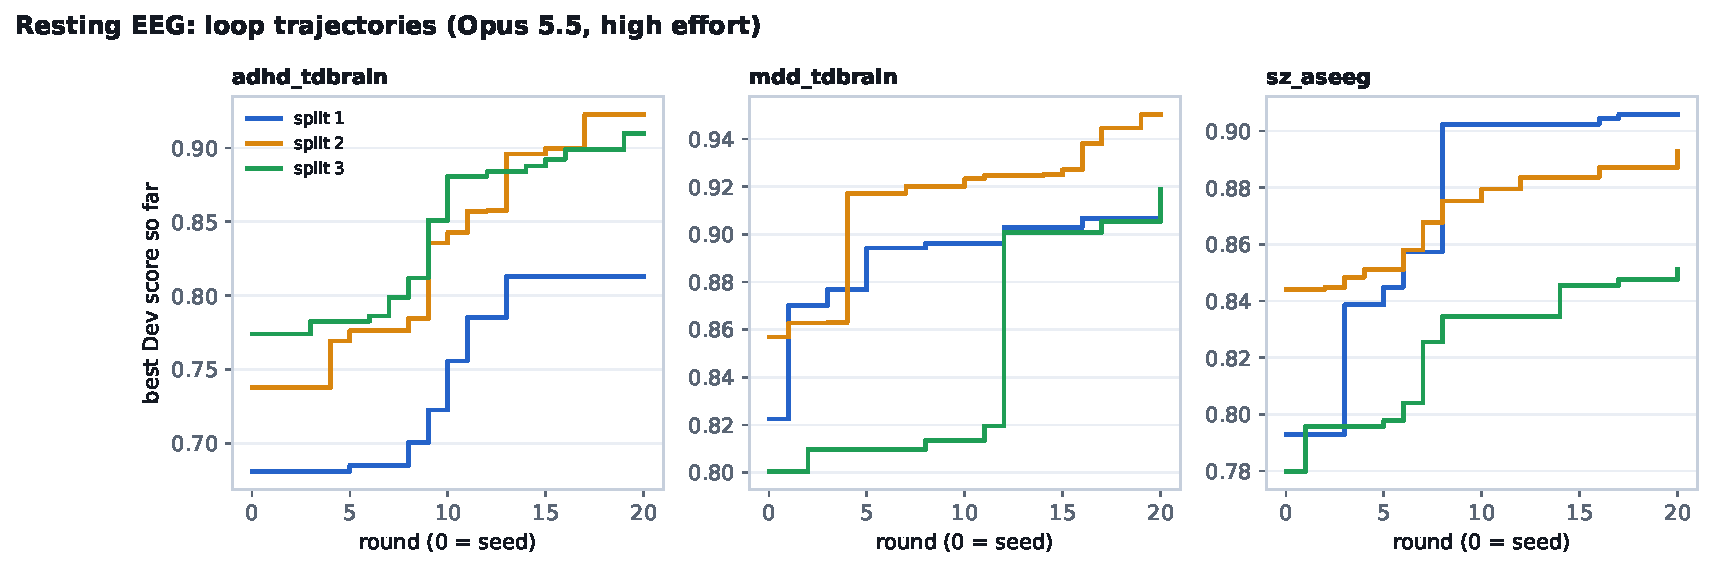
\includegraphics[width=\linewidth]{fig3_trajectories_eeg_psych.pdf}
\caption{Best Dev score so far per round, scalp EEG tasks.}
\end{figure}
\begin{figure}[htbp]
\centering
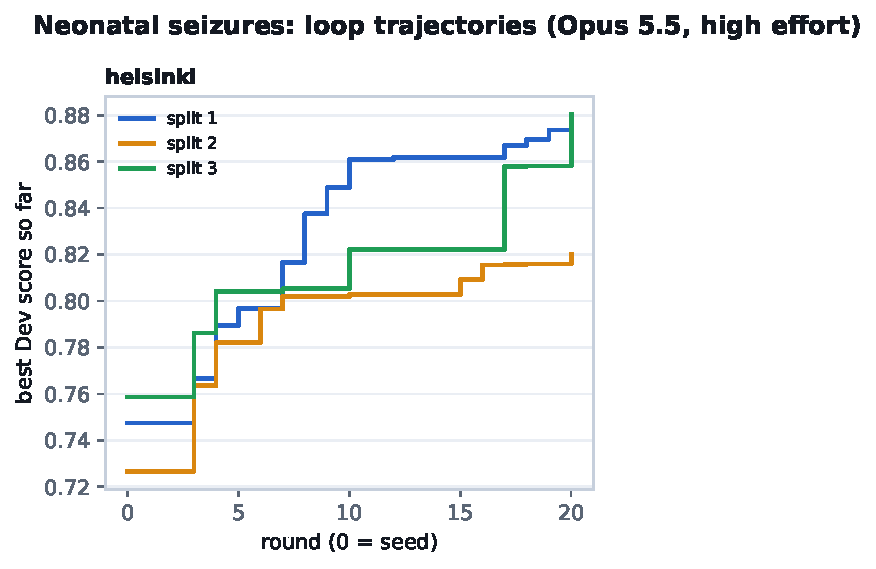
\includegraphics[width=\linewidth]{fig3_trajectories_neonatal_seizure.pdf}
\caption{Best Dev score so far per round, neonatal seizure detection.}
\end{figure}
\begin{figure}[htbp]
\centering
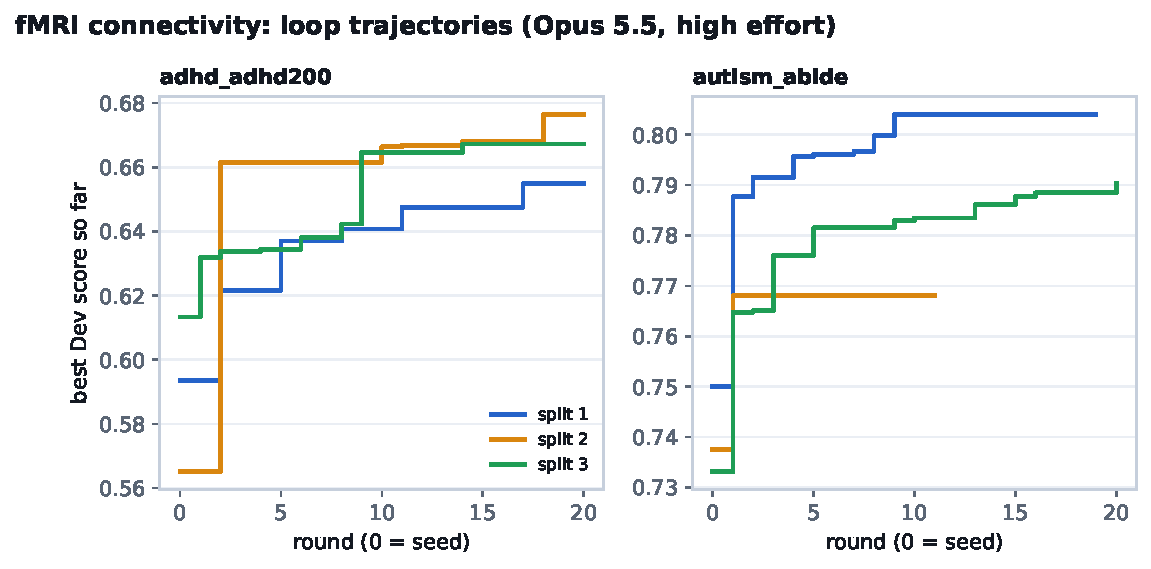
\includegraphics[width=\linewidth]{fig3_trajectories_fmri_connectivity.pdf}
\caption{Best Dev score so far per round, fMRI connectivity tasks.}
\end{figure}
\begin{figure}[htbp]
\centering
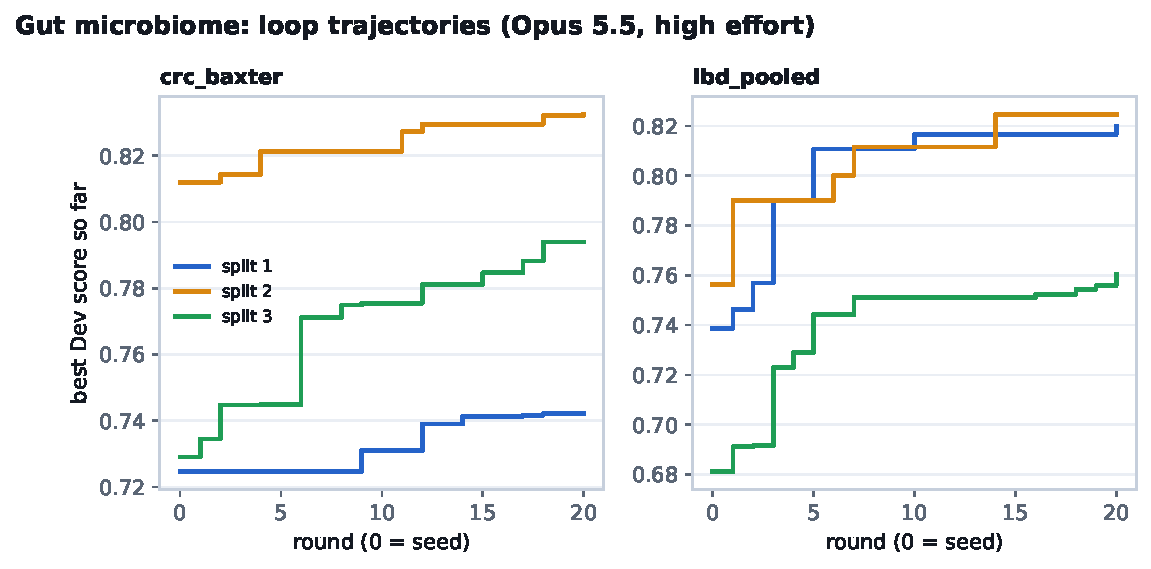
\includegraphics[width=\linewidth]{fig3_trajectories_microbiome.pdf}
\caption{Best Dev score so far per round, gut microbiome tasks.}
\end{figure}
\begin{figure}[htbp]
\centering
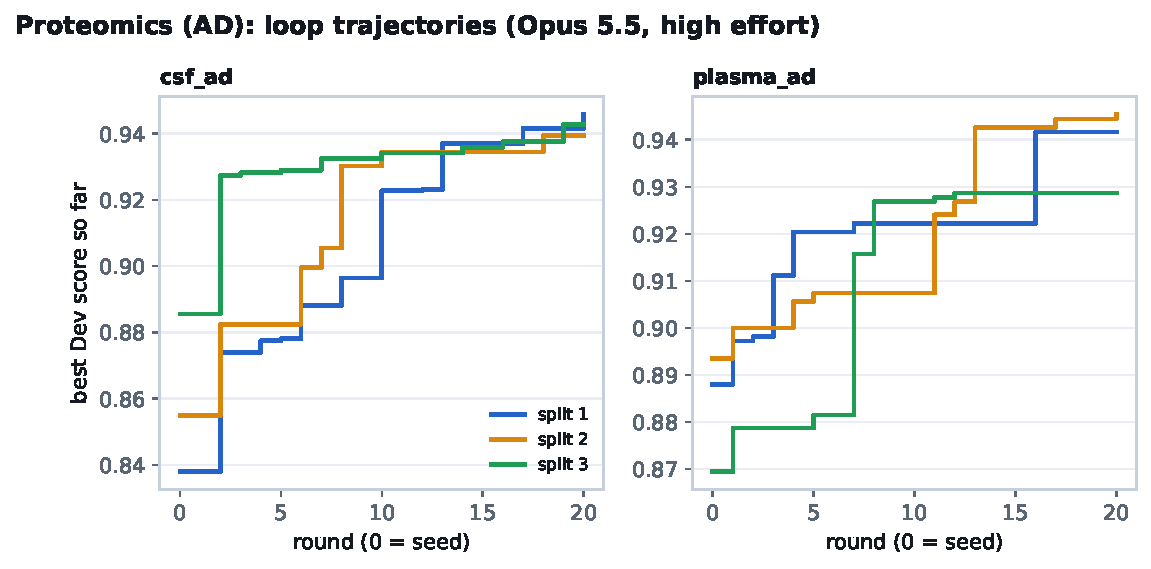
\includegraphics[width=\linewidth]{fig3_trajectories_proteomics_ad.pdf}
\caption{Best Dev score so far per round, proteomics (AD) tasks.}
\end{figure}
\begin{figure}[htbp]
\centering
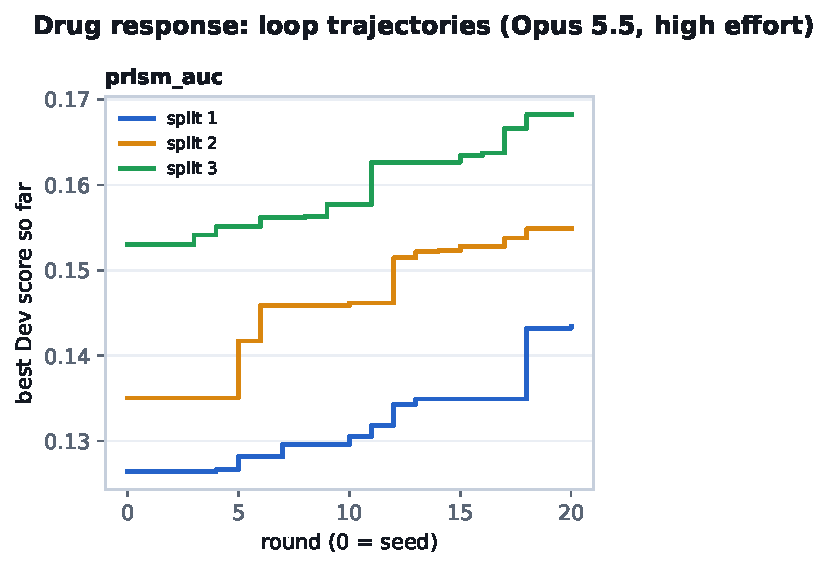
\includegraphics[width=\linewidth]{fig3_trajectories_drug_response.pdf}
\caption{Best Dev score so far per round, drug response.}
\end{figure}

\end{document}
